\section{Method} \label{sec:method}

In this section we will describe the method we have used to solve the authorship
verification problem presented in Definition \ref{def:authorship_verification}.
In general there are two methods for representing each author. There is the
\textit{instance based approach} and the \textit{profile based approach}. In
the instance based approach each author $\alpha \in \mathcal{A}$ is represented
by a set of texts $T_\alpha$ he/she have written. In the profile based approach
texts in $T_\alpha$ are combined in some way, resulting in a single (typically
smaller) ``profile'' representing the author. The instance based approach is
illustrated in Figure \ref{fig:instance_based} and the profile based approach is
illustrated in Figure \ref{fig:profile_based}.

\begin{figure}[htb]
    \centering
    \textbf{Instance Based Authorship Verification}\par\medskip
    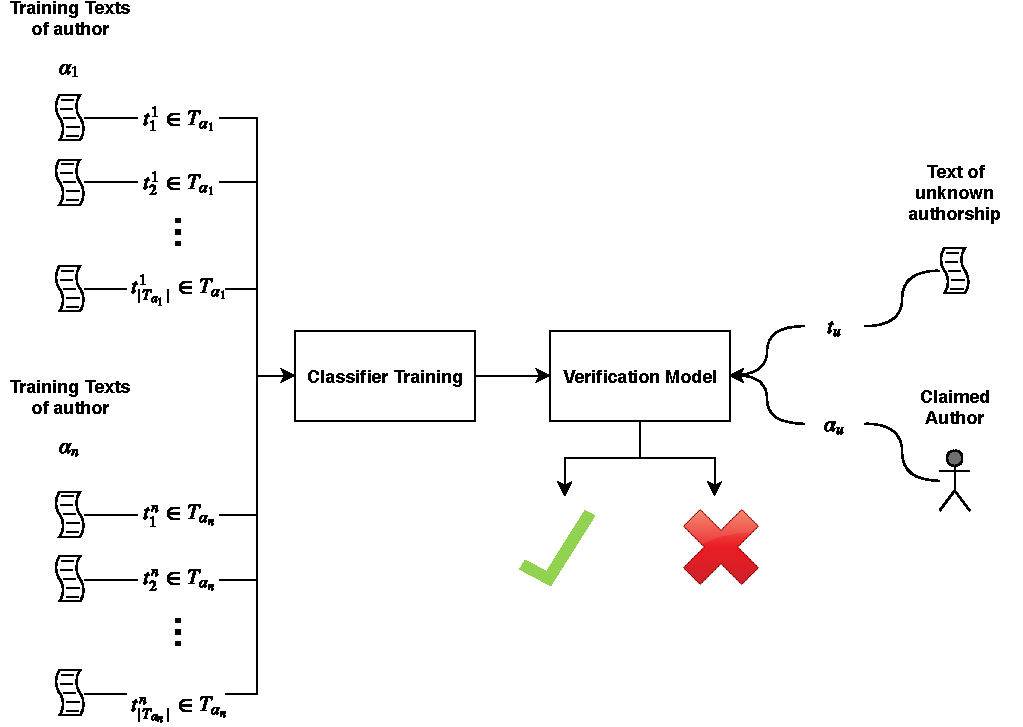
\includegraphics[width=\textwidth]{./pictures/method/instance_based}
    \caption{Illustrate the typical instance based authorship verification
    setup inspired by \citet{stamatos2009}. A set of authors are given
    as input each with a set of texts. Some machine learning model is trained on
    the input texts and the model is used to predict an unknown text $t_u$
    against a claimed author $\alpha_u$.}
    \label{fig:instance_based}
\end{figure}

\begin{figure}[htb]
    \centering
    \textbf{Profile Based Authorship Verification}\par\medskip
    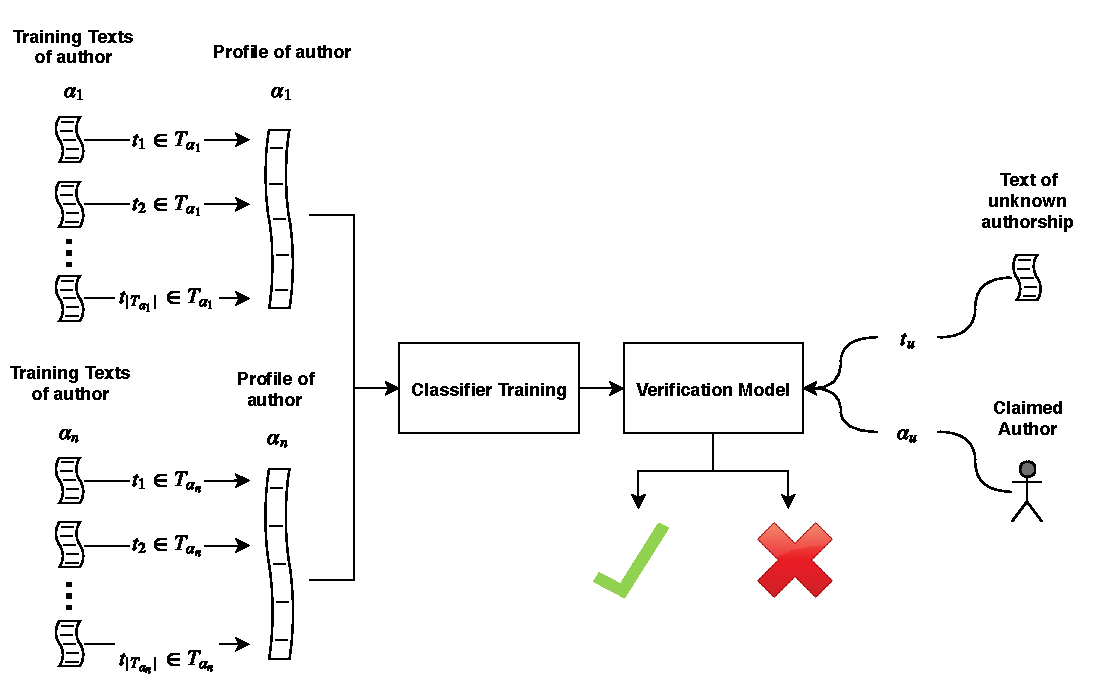
\includegraphics[width=\textwidth]{./pictures/method/profile_based}
    \caption{Illustrate the typical profile based authorship verification setup
    inspired by \citet{stamatos2009}. The texts of each author are combined
    using some combination function such as an average or a concatenation. Those
    \textit{profiles} are then given to a Machine Learning model to train. The
    output is a model which is used to predict unknown texts $t_u$ against
    claimed authors $\alpha_u$.}
    \label{fig:profile_based}
\end{figure}

An example of a profile-based authorship attribution approach which is highly
regarded by \citet{stamatos2009} use a compression algorithm. It works by
representing each author as a concatenation of all of his/her texts. The profile
of an author $\alpha$ is then the concatenation of all $t \in T_\alpha$.
Authorship of a newly introduced text is then determined by looping through each
author adding the new text to their concatenated profile. The profile is then
compressed both with and without the new text included. The bit-wise difference
is then computed by subtracting them from one another resulting in what is
essentially the cross-entropy between the two sets. The author with the lowest
cross-entropy is then considered to be the author of this new text. Different
methods of compression can be used as the base for this model each giving
different results. In the instance that \citet{stamatos2009} describes RAR
compression yielded the best results, but the choice of compression algorithm
depends on the specific scenario.

We generally use the instance based approach since it allows us to use more
metadata text information. For example the writing style of an author may change
over time especially for secondary school students that evolve a lot throughout
their school attendance. Since we use an instance based approach we are able
to weigh similarity to newer texts higher than similarity to older texts as
\citet{hansen2014} found worked well. The practical application of this will be
explained in Section \ref{subsec:combining_neural_network_output}.

There are also another split between methods that we consider. There are
generalizing and author specific models. In a generalizing model only a single
model is trained on data from multiple authors and are able to make predictions
for previously unseen authors. In the author specific model a separate model has
to be trained for each author and is not able to make predictions for previously
unseen authors. The generalizing models' main advantage is that it only has to
be trained once and after that it can be used for everyone. The author specific
model has the advantage that it can better fit to the specific quirks of a
particular author since it is trained separately for each author. We will focus
on the generalizing approach since it is more practical for MaCom as they only
have to train the model once.

In order to measure the quality of our models we will compute the number
of \glspl{TP}, \glspl{TN}, \glspl{FP} and \glspl{FN}. In the authorship
verification problem we determine whether or not a \textit{claimed} (or
\textit{candidate}) author has written a text $t$. If we determine that the
claimed author \textbf{has} written the assignment we report \textit{True} and
if we determine that the claimed author has \textbf{not} written the assignment
we report \textit{False}. Therefore we get,

\begin{itemize}
    \item a \gls{TP} whenever we answer \textbf{True} and the text \textbf{is}
        written by the claimed author,
    \item a \gls{TN} whenever we answer \textbf{False} and the text is
        \textbf{not} written by the claimed author,
    \item a \gls{FP} whenever we answer \textbf{True} and the text is
        \textbf{not} written by the claimed author, and
    \item a \gls{FN} whenever we answer \textbf{False} and the texts \textbf{is}
        written by the claimed author.
\end{itemize}

Given those definitions the \gls{TPR}, \gls{FPR}, \gls{TNR} and \gls{FNR}
are defined as follows.

\begin{definition}[\glsdesc{TPR}]

    The fraction of positives that we reported \textit{True} on i.e. the
    fraction of texts written by the claimed author that we say are written by
    the claimed author. The \gls{TPR} is computed as,

    \begin{equation}
        TPR = \frac{TP}{TP + FN}.
    \end{equation}

\end{definition}

\begin{definition}[\glsdesc{TNR}]

    The fraction of negatives that we reported \textit{False} on i.e. the
    fraction of texts not written by the claimed author that we say are not
    written by the claimed author. The \gls{TNR} is computed as,

    \begin{equation}
        TNR = \frac{TN}{TN + FP}.
    \end{equation}

\end{definition}

\begin{definition}[\glsdesc{FPR}]

        The fraction of negatives that we reported \textit{True} on i.e. the
        fraction of texts not written by the claimed author that we say are
        written by the claimed author. The \gls{FPR} is computed as,

        \begin{equation}
            FPR = \frac{FP}{FP + TN}.
        \end{equation}

\end{definition}

\begin{definition}[\glsdesc{FNR}]

    The fraction of positives that we reported \textit{False} on i.e. the
    fraction of texts written by the claimed author that we say are not written
    by the claimed author. The \gls{FNR} is computed as,

    \begin{equation}
        FNR = \frac{FN}{FN + TP}.
    \end{equation}

\end{definition}

Using these definitions we can also describe the accuracy measure we will be
reporting on throughout our experiments,

\begin{equation}
    \text{Accuracy} = \frac{TP + TN}{TP + FP + TN + FN}.
\end{equation}

Another important measurement is the accusation error. The accusation error is
given by,

\begin{equation}
    \text{Accusation Error} = \frac{FN}{FN + TN}.
\end{equation}

The goal is to keep this error under a certain threshold specified by MaCom
which is $0.1$ or $10\%$. In other words only 10\% of the accusations we make
are allowed to be wrong. In order to accommodate this constraint we can take
certain actions which depends on the model used. Details about these actions
will be addressed in Section \ref{subsec:combining_neural_network_output}.

In addition to the constraint on the accusation error Macom also wants a
specificity above 95\%. Specificity is defined as,

\begin{equation}
    \text{Specificity} = \frac{TN}{TN + FP}.
\end{equation}

Specificity therefore represents the fraction of the total negatives we catch.
To catch 95\% of ghostwriters is a very ambitious goal. As described earlier
it is more important to keep the accusation error low than to catch many
ghostwriters. We will therefore primarily focus on keeping the accusation error
lower than 10\% and then see how high we can get the specificity at the same
time.

\subsection{Baseline Methods}

We have implemented two baselines to compare with our neural network methods.
The methods were selected based on our previous work \citep{US}. The methods
were developed for English texts and not Danish texts that we work with in
this assignment. They do however represent classical machine learning methods
for solving the authorship verification problem \citep{stamatos2009}. They
will therefore serve as a great baseline for our neural networks. We believe
that by changing the parameters of the models they will work just as well for
Danish texts as they did on English texts. The Danish and English language is
very similar as they both derive from the Germanic branch of the Indo-European
language family. \citet{konstantin:2000} conducted a study of the similarities
and differences between various European languages. Based on a lexical distance
computation he determined that English and Danish are very similar.

None of the baseline methods work on raw texts. Rather they require hand
engineered feature sets extracted from the texts. The features used by
\citet{US} were all n-gram frequencies as in many classic authorship
verification methods \citep{stamatos2009}. We use the same features as
described in our previous report. We change the specific n-grams to n-grams
extracted from Danish texts but the classes of n-grams will stay the same.
The n-grams come from several linguistic layers. Specifically we use
frequencies of character-n-grams, special-character-n-grams, word-n-grams and
\gls{POS}-tag-n-grams.

\begin{description}

    \item[Character-n-gram]

        Refer to character sequences of size $n$.

    \item[Special-character-n-grams]

        Refer to sequences of characters of size $n$ where all alphanumeric and
        space characters has been removed from a text. Special-character-n-grams
        can for example be used to find authors that use long sentences and
        therefore many commas in a row.

    \item[Word-n-grams]

        Refer to sequences of words of size $n$.

    \item[\gls{POS}-tag-n-grams]

        Refer to \gls{POS}-tag sequences of size $n$. A \gls{POS}-tag is the
        grammatical class of individual words such as nouns of adjectives. To
        extract \gls{POS}-tags from texts we use the \gls{POS}-tagger provided
        by \citep{polyglot}.

\end{description}

We now shortly describe the two baseline methods we implemented.

\subsubsection{Extended Delta Method}

One of the best performing methods of \citet{US} was the extended delta
method. As the name suggests the method extends the classic delta method
\citep{evert2015towards}. The classic delta method verifies authorship of a text
by using a \gls{KNN} classifier. This \gls{KNN} is applied to a set of linearly
transformed word frequencies. The word frequencies used are the frequencies of
the $n$ most frequent words. So the \gls{KNN} is trained using the frequency
of a number of the most frequent words. The amount of most frequent words to
include can differ the amount chosen by \citep{evert2015towards} was 150.
The linear transformation he applied was a simple 0 mean and unit variance
transformation.

The extension we applied to this method, is simply to use features that are
not word frequencies. As mentioned we used this approach in our earlier work
\citep{US}. However, due to data-specific circumstances we were not able to
modify the K in \gls{KNN}. In these circumstances that is not the case. This
leaves the extended delta method with 3 configurable parameters. The features
used, how many neighbor to consider (denoted $K$), and what distance measure to
use (denoted $p$). Where $p$ is the argument used when calculating the Minkowski
distance. when $p = 1$ the Minkowski distance corresponds to the Manhattan
distance and when $p=2$ it corresponds to the Euclidean distance.

\subsubsection{Author Specific SVM}
\glsreset{SVM} 

Our other baseline method is the author specific \gls{SVM}. The method
was used in \citep{US} and was originally inspired by \citet{hansen2014}.
They used an \gls{SVM} on the Macom dataset as we described in Section
\ref{subsec:previous_work_using_macoms_dataset}. To verify the authorship of a
text $t$ and author $\alpha$ using this method, a two class \gls{SVM} classifier
has to be trained. The positive class is represented by features of each $t' \in
T_\alpha$ and the negative class is represented by the features of $t'' \in T$
where $T \subset \overline{T_\alpha}$ and $|T| = |T_\alpha|$. After training,
the classifier is used to predict if $t \in T_\alpha$ or $t \in T$.
Since a separate \gls{SVM} model is trained for each author it can learn
the specific author's writing style from $T_\alpha$. In contrast it also learns
how the author does not write using $T$.

The method is based on an \gls{SVM} so we have to experiment
with the hyperparameters $C$ and $\gamma$ \citep[E-Chapter
8]{Abu-Mostafa:2012:LD:2207825}. We find the best parameters via cross
validation. The parameter search be described in detail in Section
\ref{sec:experiments}.


\subsection{Deep Learning}

In this paper we approach the authorship verification problem using deep
learning. The term was first introduced to machine learning in 1989. The
term deep learning quickly became synonymous with neural networks as
they were some of the more efficient and popular deep learning methods
\citep{Schmidhuber:2015}.

With the inner workings of the brain used as the basis. A standard simple neural
network consists of a set interconnected processors, \textit{neurons}. Each of
these neurons has a real valued activation associated with it which activates
differently depending on the specific neuron and input. A special set of neurons
known as input neurons activate through perceiving the environment. Other
neurons are simply activated through the weighted output of previous neurons
\citep{DBLP:journals/corr/Schmidhuber14}.

Neural networks have been around since the 1940s. However, back then they
were merely variations of the linear regressors used at the time and were
not very similar to the networks we see today. It was not until the late
1960s and early 1970s, that networks comparable to the more modern approaches
surfaced. Examples of such early works are \citep{ivakhnenko1973cybernetic}
and \citep{4308320} which describe multi-layered feed forward supervised
neural network architectures. While the work described by those two authors
looked like modern neural networks architecture wise they had large problems
with updating the weights in the network efficiently. The basics of continuous
\textit{backpropagation} was initially described by \citet{Kelley1960}
quickly followed by a simpler approach which used only the chain rule
by \citet{DREYFUS196230}. It was not until 1970 that the modern version
of backpropagation was described using automatic differentiation. This
prompted an increase in backpropagation related research in the following
decades. As computational power increased in the 1990s and 2000s, so did
the practical usage of backpropagation and neural network in general
\citep{Schmidhuber:2015}. The theory behind backpropagation will be described in
Section \ref{subsubsec:training_a_network}.

\glsreset{CNN} 

Like with the history of authorship verification, research in this area of
science picked up more interest as we entered the modern computational age and
with the introduction of the \gls{CNN}. \glspl{CNN} are based on the early work
described in \citet{TJP:TJP19681951215}. They showed that cats' and monkeys'
visual cortices contain a set of neurons each individually responding to a
receptive field (area) of their field of view. Neightboring receptive fields
all have a certain amount of overlap but in the end a cohesive view is created.
This is what paved the way for neocognition in 1980 \citep{Fukushima1980},
the basis of \glspl{CNN} which looks at overlapping subsections of data
\citep{Schmidhuber:2015}.


\subsubsection{Neurons}\label{sec:neurons}

As mentioned previously a neural network consists of a collection of neurons.
Each neuron is a simplified mathematical model which behaves much like neurons
in the brain. They receive, process and transmit information. Each neuron has a
set of inputs called $x_{j}$ one of which, $x_{0}$, is a special bias input set
to 1 and a single output called $z_i$, where $i$ refers to the neuron and $j$
refers to a specific input to that neuron. Each neuron computes a weighted sum
of its inputs and applies an activation function $h$ to the weighted sum. The
weights are called $w_{ij}$ and the weight of the bias $w_{i0}$. The function
each neuron computes is,

\begin{equation}\label{eq:neuron}
    z_i = h(a_i) = h\left(
        \sum_{j = 1}^d w_{ij}x_j + w_{i0}
 \right) = h\left(
        \sum_{j = 0}^d w_{ij}x_j \right)
\end{equation}

where $d$ is the number of inputs to the neuron. A more intuitive model of such
a neuron can be seen in Figure \ref{fig:neuron}.

\begin{figure}[!tbp]
  \centering
  \begin{minipage}[b]{0.45\textwidth}
    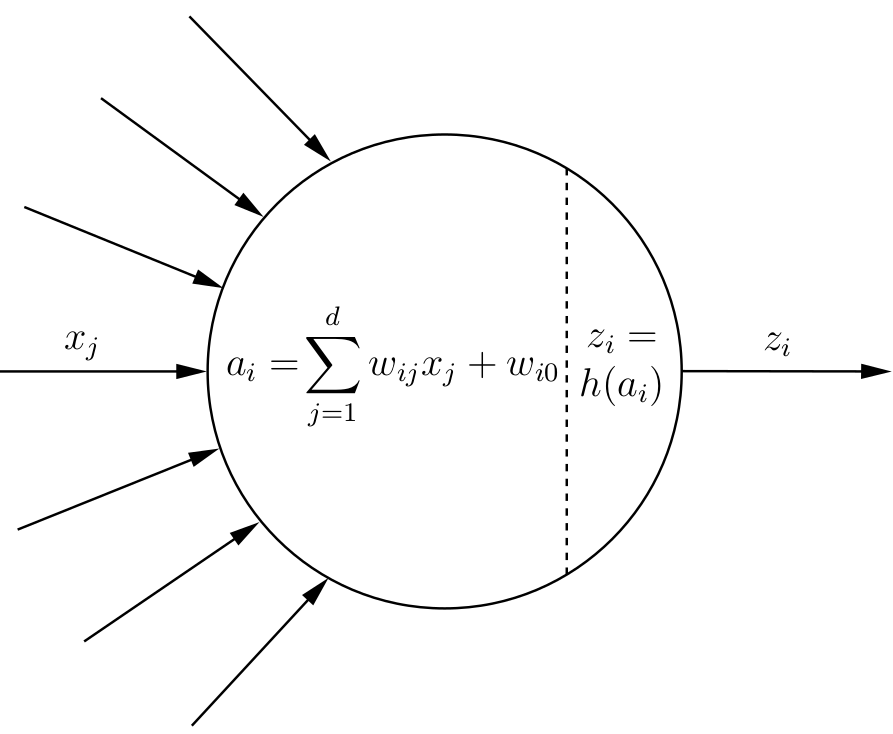
\includegraphics[width=\textwidth]{./pictures/method/neuron.png}
  \end{minipage}
  \hfill
  \begin{minipage}[b]{0.45\textwidth}
    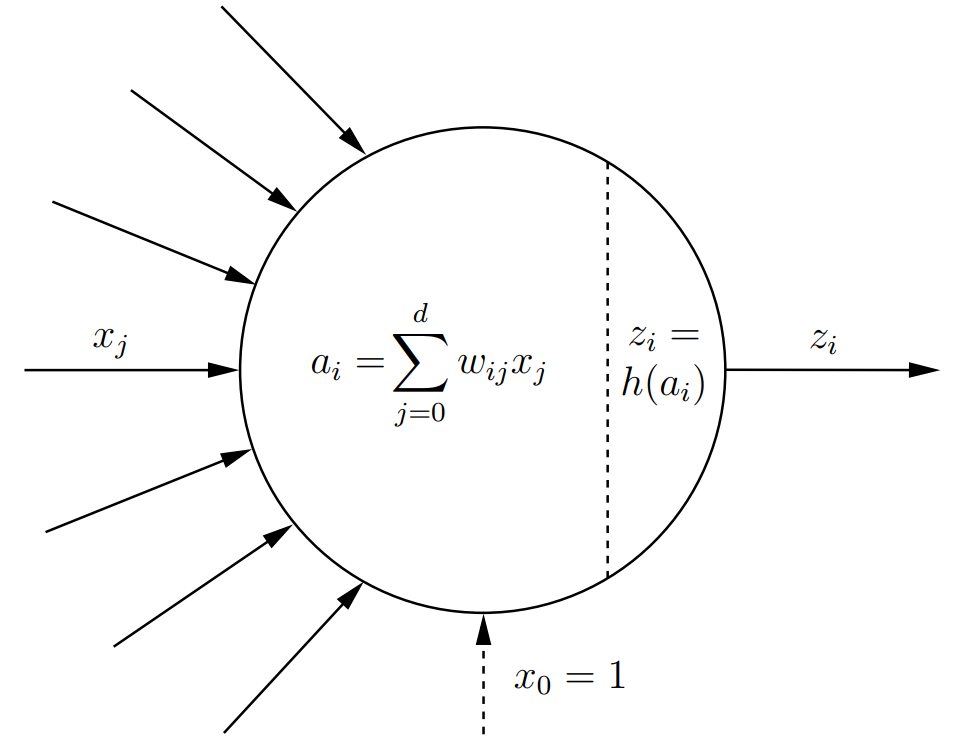
\includegraphics[width=\textwidth]{./pictures/method/neuron_bias.png}
  \end{minipage}
    \caption{The inner workings of a neuron, with and without an implicit
        bias \citep{Igel}. The left figure is without implicit bias while the
        right figure is with implicit bias.}
\label{fig:neuron}
\end{figure}

Neurons are usually arranged in layers in order to achieve a certain desired
behaviour. More details regarding these layers will be explained in Section
\ref{subsubsec:layers}. The training of a neural network consists of changing
the weights applied at each neuron, with the goal of modeling the relationships
present in the data.


\subsubsection{Activation Functions} \label{subsubsec:activation_functions}

The activation function $h$ of a neuron is applied to the output of the
neuron. Activation functions are typically non linear functions as that allows
for the network to compute more complex functions \citep{6797088}. A plot
of classic activation functions used in neural networks is shown in Figure
\ref{fig:activation_functions}.

\begin{figure}
    \centering
    \textbf{Activation Functions}\par\medskip
    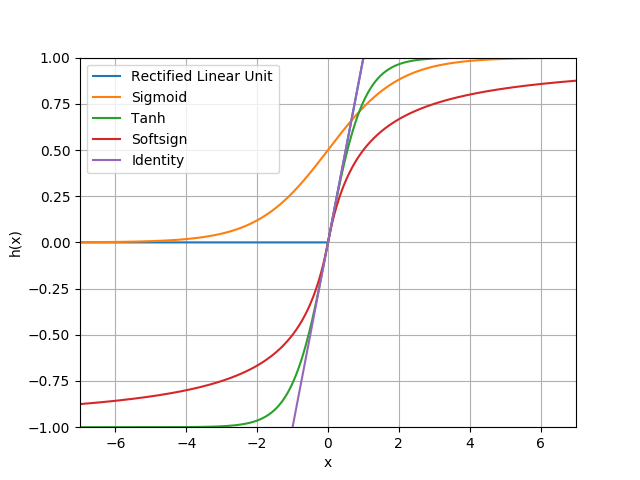
\includegraphics[width=0.5\textwidth]{./pictures/method/activation_functions.png}
    \caption{Different activation functions that can be used in neural
        networks.}
    \label{fig:activation_functions}
\end{figure}

Each activation function has advantages and disadvantages. We mainly used the
\gls{ReLu} activation function in the layers of our networks - it is defined
as such,

\begin{equation}
    h(x) = \max(0, x)
\end{equation}

\gls{ReLu} is generally considered a general purpose activation function. When
selecting an activation function for your neurons, the best function would be
the one which best approximates the underlying data relationship. Without a good
idea as to what that function might be \gls{ReLu} is a good starting point. Its
simplicity, quick computation time and its below zero limitation means that
a large portion of the network will not be activating, resulting in an even
smaller computation time. In addition to that, the derivative of the function
is 1 in the case of a positive input resulting in the backpropagation loss
having equal influence throughout the network. In the case of other activation
functions that might not be the case resulting in an altering of the error as
we propagate backwards through the network. This can lead to a big error in the
deeper layers not reaching the shallow layers of the network. This property of
the \gls{ReLu} activation function does not come without costs. If the learning
rate of the network is not configured correctly a \gls{ReLu} activated neuron
might be blasted with a gradient so large that it never reaches a point of
activation again. In other words, the neuron "dies". As such, one can risk a
network containing a lot of dead non-activating neurons greatly decreasing its
learning power. On the other hand there is sigmoid activation function,
which is defined as follows, 

\begin{equation}
    h(x) = \frac{1}{1 + e^{-x}}
\end{equation}

This activation function does not allow its neurons to die. It can become
victim to saturation. In the case of a weight being too small or too large, the
output values will be placed at the far ends of the sigmoid range of values.
At this point the gradient is incredibly small meaning that the contribution
that neuron now has is negligible. This neuron is now only a strain on the
network, slowing it down through its activation but contributing nothing - a
problem \gls{ReLu} does not have. Its based on these considerations we chose the
\gls{ReLu} activation function, leaving us the task of properly selecting our
learning rate \citep{JiYan, AndrejKarpathy, AvinashSharmaV}.

Exceptions to usage of the \gls{ReLu} activation function can be found when
we use \gls{LSTM} layers during our experimentation. There we used the tanh
activation function,

\begin{equation}\label{eq:tanh}
    h(x) = \tanh(x) = \frac{(e^x - e^{-x})}{(e^x + e^{-x})},
\end{equation}

and the hard sigmoid activation function,

\begin{equation}\label{eq:h_sig}
    h(x) = \max(0, \min(1, x \cdot 0.2 + 0.5)).
\end{equation}

These both serve as the default activations functions when using the Keras
deep learning library, which is what we used to produce this system.
\cite{chollet2015keras}.

As the activation function of our output neurons we have used the softmax
function. The function is defined as

\begin{equation}
    h(x_i) = \frac{e^{x_i}}{\sum_{k=1}^n e^{x_k}}, \text{for $i = 1,\dots,n$}.
\end{equation}

The softmax function takes any vector $x \in \mathbb{R}^n$ and returns a vector
$y \in [0, 1]^n$. Where the sum of the output vectors elements will be equal to
1. The function is therefore great at constructing a probability distribution
based on an input vector.

\subsubsection{Layers} \label{subsubsec:layers}

Neural networks are organized in layers of neurons. The first layer is called
the input layer and is connected directly to the input of the model and the last
layer is called the output layer. The output of this layer is considered the
output of the entire network. All layers in between are called hidden layers. A
practical example could be an the input layer where each neuron were connected
to a pixel of an image. The output layer could then consist of a single neuron
that computes the probability that the picture contained a cat. An example of
such a layered neural network are shown in Figure \ref{fig:example_nn}.

\begin{figure}
    \centering
    \textbf{Example Neural Network}\par\medskip
    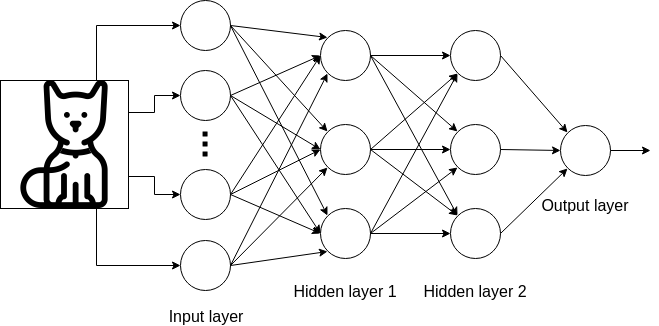
\includegraphics[width=\textwidth]{./pictures/method/example_neural_network}
    \caption{Example neural network that illustrates how neurons are organized
        into different layers with a special input layer, a special output layer
        and two hidden layers. The neurons in the input layer are connected to
        individual pixels in an input image and the output layer is a single
        neuron computing the probability that the image contains a cat.}
    \label{fig:example_nn}
\end{figure}

There are different kinds of layers. Below is a
non-exhaustive description of different layers, based on
\citep{oshea2015,DBLP:series/sci/2012-385,Goodfellow-et-al-2016,
mikolov2013linguistic,JMLR:v15:srivastava14a}:

\begin{description}

    \item[Dense Layer:]

        In a dense layer the input of each neuron in the layer is connected to
        the output of every neuron in the previous layer. Each neuron in the
        layer computes a weighted sum of the outputs of the previous layers'
        neurons and applies an activation function. The weights for each of
        the neurons in the layer are different allowing each neuron to learn a
        different combination of the previous layer. An example of this can be
        seen in Figure \ref{fig:example_nn}, where the hidden layers are dense.

    \item[Convolutional Layer:]

        A convolutional layer is mainly used to extract position independent
        features from data. The convolution consist of a sliding window that
        slides over some input data and gives an output for each possible
        position in the input. The sliding window use the same weights
        in all the positions and will therefore extract the same features from
        different locations if it is presented with the same input. The
        convolution computes a single output for each window position. The
        output is computed as the sum of the elementwise multiplication of
        the sliding window and the current part of the input it is looking at
        \citep{oshea2015}. Let us for example consider a two dimensional input,

        \begin{equation}
            X = \begin{pmatrix}
                1 & 1 & 1 & 0 \\
                1 & 0 & 0 & 1 \\
                0 & 1 & 0 & 1 \\
                0 & 0 & 1 & 0
            \end{pmatrix},
        \end{equation}

        and the convolutional filter,

        \begin{equation}
            w = \begin{pmatrix}
                1 & 0 & 0 \\
                1 & 0 & 0 \\
                0 & 1 & 0 \\
            \end{pmatrix}.
        \end{equation}

        Then we start the sliding window in the top left corner and compute the
        elementwise product of the matrices,

        \begin{equation}
            Y = X_{[1,3;1,3]} \otimes w =
            \begin{pmatrix}
                1 & 1 & 1 \\
                1 & 0 & 0 \\
                0 & 1 & 0
            \end{pmatrix} \otimes
            \begin{pmatrix}
                1 & 0 & 0 \\
                1 & 0 & 0 \\
                0 & 1 & 0
            \end{pmatrix} =
            \begin{pmatrix}
                1 & 0 & 0 \\
                1 & 0 & 0 \\
                0 & 1 & 0
            \end{pmatrix},
        \end{equation}

        to then compute the final value we take the sum of all the elements in
        that matrix,

        \begin{equation}
            \sum_{i,j} Y_{i,j} = 1 + 0 + 0 + 1 + 0 + 0 + 0 + 1 + 0 = 3.
        \end{equation}

        We then slide the window one to the right and repeat the same process,

        \begin{equation}
            Y = X_{[2,4;1,3]} \otimes w =
            \begin{pmatrix}
                1 & 1 & 0 \\
                0 & 0 & 1 \\
                1 & 0 & 1
            \end{pmatrix} \otimes
            \begin{pmatrix}
                1 & 0 & 0 \\
                1 & 0 & 0 \\
                0 & 1 & 0
            \end{pmatrix} =
            \begin{pmatrix}
                1 & 0 & 0 \\
                0 & 0 & 0 \\
                0 & 0 & 0
            \end{pmatrix},
        \end{equation}

        and the final value,

        \begin{equation}
            \sum_{i,j} Y_{i,j} = 1.
        \end{equation}

        We keep sliding the window right until we run out of input. After that
        we go back to the left and go one row down. We continue the process for
        all the input and we end up with the matrix,

        \begin{equation}
            O = \begin{pmatrix}
                \sum_{i,j} \left( X_{[1,3;1,3]} \otimes w \right)_{i,j} &
                \sum_{i,j} \left( X_{[2,4;1,3]} \otimes w \right)_{i,j} \\
                \sum_{i,j} \left( X_{[1,3;2,3]} \otimes w \right)_{i,j} &
                \sum_{i,j} \left( X_{[2,4;2,3]} \otimes w \right)_{i,j}
            \end{pmatrix} = \begin{pmatrix}
                3 & 1 \\
                1 & 2
            \end{pmatrix}.
        \end{equation}

        A visualization of this process can be seen in Figure
        \ref{fig:convolution_visualization}.

        \begin{figure}
        \centering
        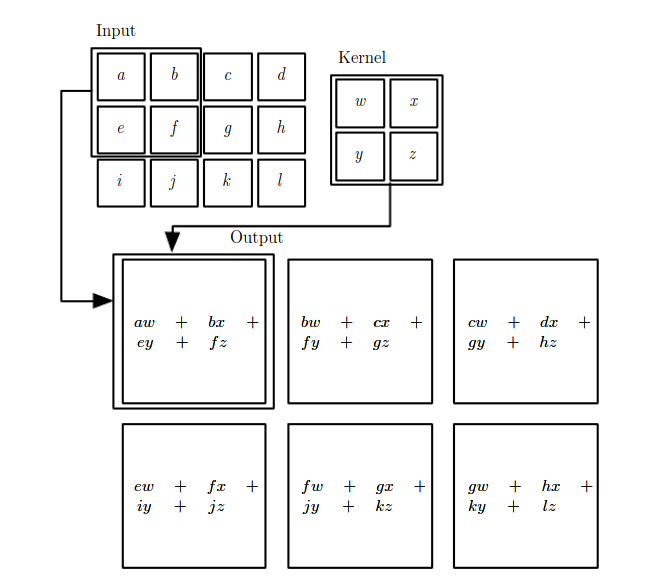
\includegraphics[width=0.6\textwidth]{./pictures/method/convolution_visualization.png}
        \caption{An example of 2D convolution, using a 2x2 kernel/sliding window
            size and a step size of 1 \citep{Goodfellow-et-al-2016}.}
        \label{fig:convolution_visualization}
        \end{figure}

        It can be seen that the output size is smaller than the input size. To
        prevent that the input can be padded with some value. A normal choice is
        zero padding. For the above input that would result in,

        \begin{equation}
            \begin{pmatrix}
                1 & 1 & 1 & 0 \\
                1 & 0 & 0 & 1 \\
                0 & 1 & 0 & 1 \\
                0 & 0 & 1 & 0
            \end{pmatrix} \xrightarrow{\text{zero padding}}
            \begin{pmatrix}
                0 & 0 & 0 & 0 & 0 & 0 \\
                0 & 1 & 1 & 1 & 0 & 0 \\
                0 & 1 & 0 & 0 & 1 & 0 \\
                0 & 0 & 1 & 0 & 1 & 0 \\
                0 & 0 & 0 & 1 & 0 & 0 \\
                0 & 0 & 0 & 0 & 0 & 0
            \end{pmatrix}.
        \end{equation}

        This would also make sure that edge values has the same amount of
        influence as the rest of the values. The sliding length can be different
        than one and is usually referred to as \textit{stride}. The weights
        the convolutional window use are learnable by the network. Certain
        convolutional filters can be used for edge detection and blurring the
        input. Some examples of different convolutional kernels applied to a
        grayscale image are shown in Figure \ref{fig:convolution_example}.

        \begin{figure}
            \centering
            \textbf{Examples of different convolutional kernels}\par\medskip
            \begin{tabular}{ccc}
                \textbf{Original} & \textbf{Kernel} & \textbf{Result} \\
                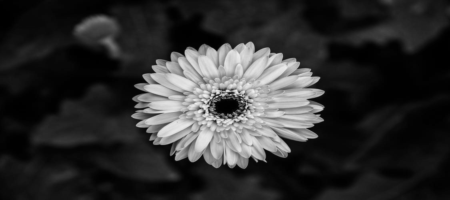
\includegraphics[width=0.3\textwidth]{./pictures/method/original_convolution.png} &
                \raisebox{1.2\height}{
                \begin{minipage}[b]{6cm}
                    \begin{equation*}
                        \begin{pmatrix}
                            1 & 0 & -1 \\
                            0 & 0 & 0  \\
                            -1 & 0 & 1
                        \end{pmatrix}
                    \end{equation*}
                \end{minipage}}
                    &
                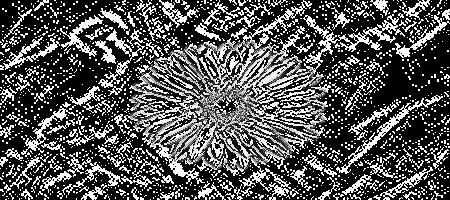
\includegraphics[width=0.3\textwidth]{./pictures/method/edge_detect_convolution.png} \\

                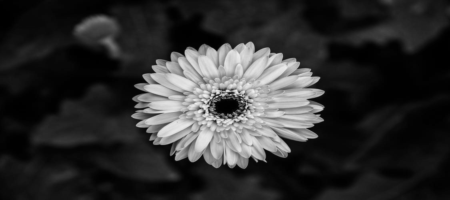
\includegraphics[width=0.3\textwidth]{./pictures/method/original_convolution.png} &
                \raisebox{1.2\height}{
                \begin{minipage}{6cm}
                    \begin{equation*}
                        \frac{1}{16}\begin{pmatrix}
                            1 & 2 & 1 \\
                            2 & 4 & 2  \\
                            1 & 2 & 1
                        \end{pmatrix}
                    \end{equation*}
                \end{minipage}}
                    &
                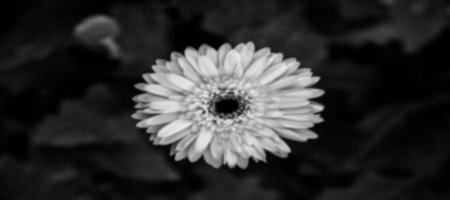
\includegraphics[width=0.3\textwidth]{./pictures/method/blurred_convolution.png} \\

                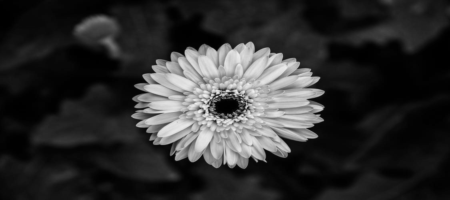
\includegraphics[width=0.3\textwidth]{./pictures/method/original_convolution.png} &
                \raisebox{1.2\height}{
                \begin{minipage}{6cm}
                    \begin{equation*}
                        \begin{pmatrix}
                            0  & -1 & 0  \\
                            -1 & 5  & -1 \\
                            0  & -1 & 0
                        \end{pmatrix}
                    \end{equation*}
                \end{minipage}}
                    &
                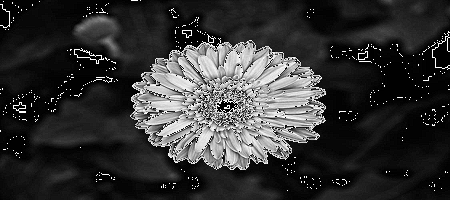
\includegraphics[width=0.3\textwidth]{./pictures/method/sharpened_convolution.png}
            \end{tabular}
            \caption{Examples of convolutional kernels applied to an image. The
                first kernel is an edge detect kernel, the second a blurring
                kernel and the third a sharpening kernel.}
            \label{fig:convolution_example}
        \end{figure}

        Convolutional layers for text analysis works slightly differently.
        Text is not two dimensional but one dimensional data. A convolution
        on text therefore does not use a two dimensional sliding window but
        a one dimensional one. The process is the same as before. The window
        slides over the text looking at a sequence of characters at a time. Each
        character is multiplied by the weight in that positition and a sum is
        computed. The output of the layer is a one dimensional sequence of these
        weighted sums. We will describe in more detail how convolutions for text
        work in Section \ref{subsubsec:conv_char_nn}.

    \item[\gls{RNN} Layer:]

        An \gls{RNN} network resembles a normal feed forward
        neural network except that it allows circular connections
        \citep{DBLP:series/sci/2012-385}. The circular connections can be used
        to remember previous inputs and an \gls{RNN} therefore has a sense of
        history of previous input and output. Classical feed forward neural
        networks can be viewed as mappings from and to vectors while \glspl{RNN}
        can be viewed as mappings from and to sequences of vectors. An \gls{RNN}
        does not view its input as a vector but as a sequence of input vectors
        in different timesteps. We have shown an example of an \gls{RNN} network
        in Figure \ref{fig:rnn_illustration}.

        \begin{figure}
            \centering
            \textbf{Illustration of an \gls{RNN} Layer}\par\medskip
            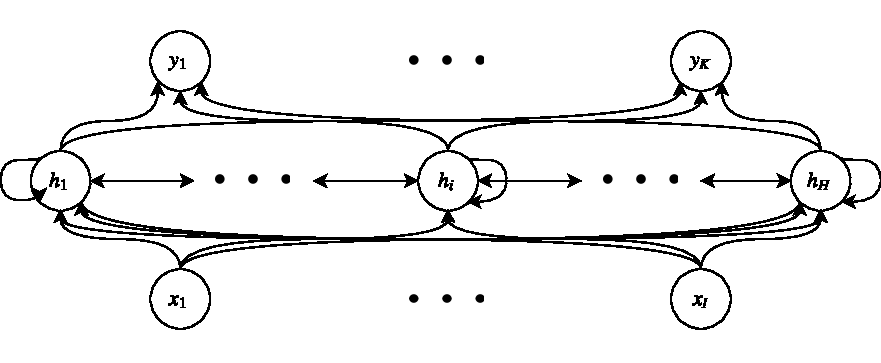
\includegraphics[width=\textwidth]{./pictures/method/RNN}
            \caption{Illustrates the structure of an \gls{RNN}. The \gls{RNN}
                consist of three layers, an input layer, a hidden layer and an
                output layer. The \gls{RNN} shown consist of $I$ input units,
                $H$ hidden units and $K$ output units. In the hidden layer each
                neuron is connected to every other neuron in the layer including
                itself and to every input neuron. In the output layer each
                neuron is connected too all hidden units.}
            \label{fig:rnn_illustration}
        \end{figure}

        In the forward pass of an \gls{RNN} network both the activations of
        the hidden units and the activations of the output units have to be
        computed. In the computation of the activation of the hidden units, the
        output of hidden units in the previous timestep are required. We let
        $a^{(t)}_h$ denote the activation of neuron $h$ in the hidden layer in
        timestep $t$. It is computed as,

        \begin{equation}
            a^{(t)}_h = \psi_h\left(
                \sum_{j=1}^I w_{hj} x^{(t)}_j +
                \sum_{h'=1}^H w_{hh'} a^{(t-1)}_{h'}
            \right),
        \end{equation}

        where $x_j^{(t)}$ is the j'th input at timestep t, $\psi_h$ is
        the activation function of the hidden unit, $I$ is the number of input
        units, $H$ is the number of hidden units and $w_{hj}$ is the weight
        between neuron $h$ and the $j$'th input to that neuron. The weight
        $w_{hj}$ and $w_{hh'}$ does not refer to the same weight even when $j =
        h'$. Instead we abuse notation such that $w_{hj}$ enumerates the weights
        between the input and hidden layer and $w_{hh'}$ enumerates the weights
        between the hidden layer neurons. That is the activation of a hidden
        unit is an activation function applied to a weighted sum of the current
        inputs and the activation of all hidden units in the previous timestep
        \citep{DBLP:series/sci/2012-385}. The output of the \gls{RNN} is then
        computed as,

        \begin{equation}
            y^{(t)}_k = \sum_{h=1}^H w_{hk} a_{h}^{(t)}.
        \end{equation}

        That is the output of an \gls{RNN} layer is a weighted sum of its
        hidden units. The complete sequence of hidden activations are computed
        by starting at time $t=1$ and calling the functions above until
        the end of the sequence is reached incrementing $t$ by one in each
        recursive call. The initial weights of the hidden units can be any
        initialization value. The obvious choice is 0, however better results
        have been found using non zero initial hidden unit weight values
        \citep{DBLP:series/sci/2012-385}.

        An \gls{RNN} is normally trained using the \emph{backpropagation through
        time} algorithm. For data where the usage of time does not make sense
        and where the context from both sides of each timesteps is useful such
        as for text it is normal to use bidirectional \glspl{RNN}. Then both a
        forward and a backward pass are made through the sequence. The output
        of each network at each time step can then depend both on the context
        before and after the input.

    \glsreset{LSTM}
    \item[\gls{LSTM} Layer:]
        \label{layer:LSTM}

        As described the main benefit of \glspl{RNN} are their ability to use
        previous context to make predictions. Unfortunately the \gls{RNN}
        architecture described above in practise does not allow context from
        far away to influence current output. The problem is known as the
        vanishing/exploding gradient problem. When backpropagating through an
        \gls{RNN} network each timestep corresponds to a separate layer in a
        normal feed forward neural network. So for sequences of several thousand
        timesteps, backpropagation has to go through several thousand layers.
        The magnitude of the gradient will at each layer either increase or
        decrease and through the hundreds or thousands of layers that results to
        the gradient either blowing up exponentially or vanishing to nothing.
        In practise the main problem is the vanishing gradient and not the
        exploding gradient. The vanishing gradient means that weights early
        in the network are not updated according to the final output since
        the gradient has disappeared while backpropagating back to the early
        weights. Therefore the network will not learn to use context over long
        periods of time but only to use the local context around a particular
        timestep \citep{DBLP:series/sci/2012-385}.

        There are several solutions to that problem and one of them are
        \gls{LSTM} networks. \gls{LSTM} networks were introduced by
        \citet{Hochreiter:1997:LSM:1246443.1246450}. \gls{LSTM} networks are
        designed to be able to remember things over long periods of time, hence
        the name. They have several \gls{RNN} constructs with specific purposes.
        They have an \gls{RNN} responsible for computing the output given the
        current input and the previous activation as described before. They have
        an \gls{RNN} responsible for deciding what part of the input to ignore.
        They have an \gls{RNN} responsible for deciding what to forget from the
        current memory. Finally they have an \gls{RNN} responsible for deciding
        what part of the output to select as the current output of the unit
        \citep{DBLP:series/sci/2012-385}. We have showed the structure of an
        \gls{LSTM} in Figure \ref{fig:lstm}.

        \begin{figure}
            \centering
            \textbf{Structure of an \gls{LSTM}}\par\medskip
            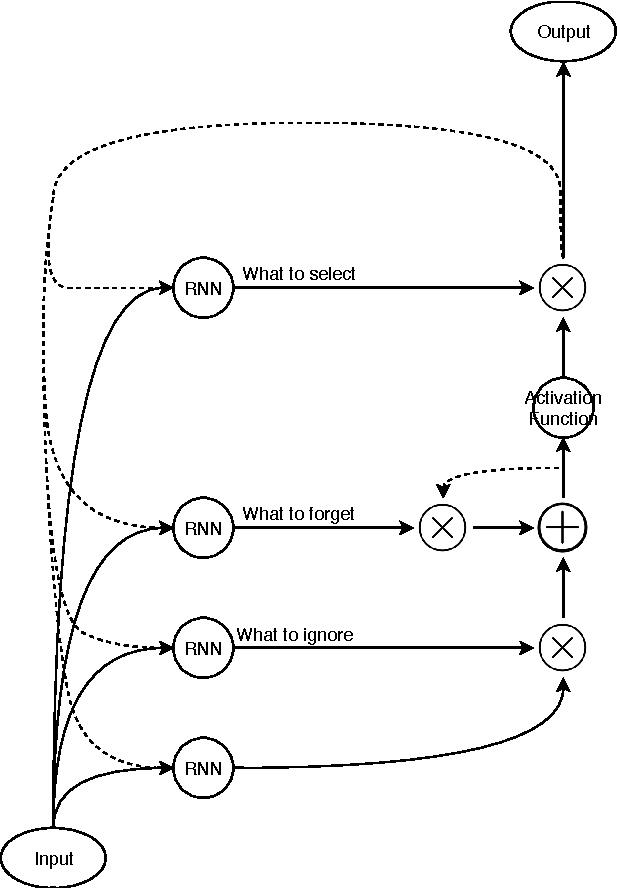
\includegraphics[scale=0.5]{./pictures/method/LSTM}
            \caption{The structure of an \gls{LSTM} network. $\bigoplus$ denotes
                an elementwise addition and $\bigotimes$ denotes an elementwise
                multiplication. Dotted lines show the movement of activations in
                the previous timestep while full lines show movement of the
                input in the current timestep.}
            \label{fig:lstm}
        \end{figure}

        The input to the \gls{LSTM} is fed into 4 \gls{RNN} networks that also
        receives the output from the previous timesteps. From bottom to top in
        the figure the \glspl{RNN} are:

        First: A network combining the current input and the previous output
        into an activation in the current timestep.

        Second: A network combining the current input and the previous output to
        compute which part of the activation of the first network to keep. The
        output of the second network is combined with the first network with an
        elementwise multiplication. That means that if the second network output
        a small value in a particular part of the output vector then that value
        will disappear from the output of the first network. The \gls{LSTM}
        therefore learns which part of the output to ignore.

        Third: A network combining the current input and the previous output
        to decide what to forget. The output of the network is combined with
        the current memory with an elementwise multiplication. So again if the
        network outputs a small value it can choose to forget a certain item.
        The network will learn when to throw things out of the current memory
        and when to keep them. The output of the elementwise multiplication is
        then combined with the current output via a elementwise addition. That
        allows the current memory to influence the output of the network. The
        added output and memory are transferred through an activation function
        that makes sure that nothing blows up and we get numerical instability.

        Fourth: A network combining the current input and the previous output
        to choose which values of the current output to select as the actual
        output. The output of the fourth network will be combined with the
        current output with an elementwise multiplication. So again the network
        can select which values to keep by outputting large numbers and which
        values to throw away by outputting small numbers. This network is the
        last applied to the output and can therefore select which values should
        be output.

    \item[Embedding:]

        The embedding layer maps a value into a continuous vector space. Given
        a sequence of one-hot encoded vectors it use the weights associated
        with the layer to map that each one-hot vector to a dense vector of
        predetermined size. This can be done on any sort of data as longs as it
        is one-hot encoded. Embedding layers are widely used in \gls{NLP}
        for mapping characters or words to dense vectors.

        The hope with using a layer such as this on characters would be that
        each character got mapped to a point close to similar characters. They
        are however mainly used to embed words. \citet{mikolov2013linguistic}
        found that embedding layers are able to learn more that just word
        similarities. They for example found that $vec("king") - vec("man") +
        vec("woman") \approx vec("queen")$ that is the embeddings learned the
        relation between the words king and queen and not just that they are
        similar words.

        \begin{figure}
            \centering
            \textbf{Example Character Embedding}\par\medskip
            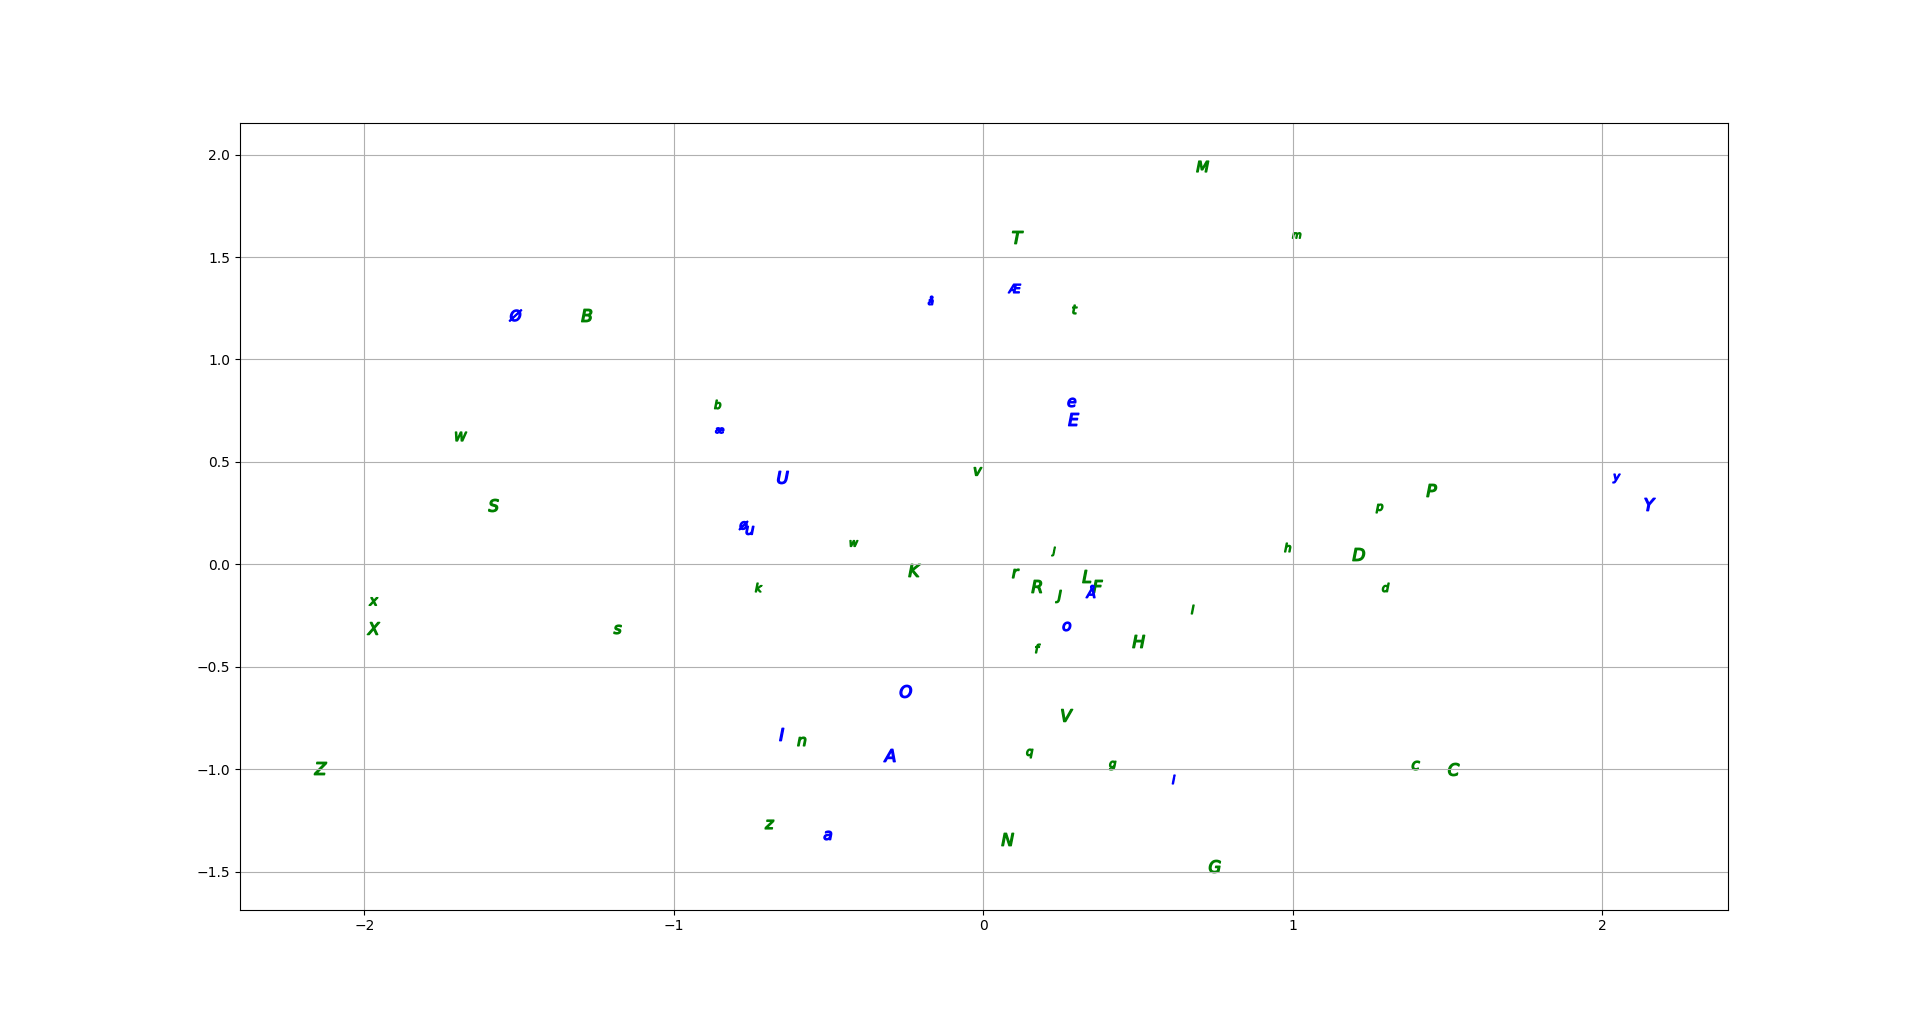
\includegraphics[width=\textwidth]{./pictures/method/example_character_embeddings.png}
            \caption{Character embeddings learned by a neural network. The
                embeddings were originally in 5 dimensional vectorspace and what
                is shown here is the first two principal components. Vowels are
                shown in blue and consonants in green.}
            \label{fig:embeddings}
        \end{figure}

        In Figure \ref{fig:embeddings} we have shown the embedding one of our
        networks produces. The characters are embedded in 5 dimensions so the
        plot shows the first two principal components only. We can see that
        several lower and upper case letters have ended up close to each other.
        That means that the network has learned that those characters are
        interchangeable.

    \item[Pooling Layer:]

        The purpose of a pooling layer, or down-sampling layer to pool the
        data it receives. It does so with the goal of distilling the data down
        to a number of key features found within said data. This of course
        decreases the computation time of the network as a whole, and with a
        smaller amount of parameters, comes a smaller chance of overfitting and
        a reduction in training time.

        One of the most used pooling layers are the max pooling layer. It works
        in similar fashion as the convolutional layer and also use a sliding
        window. This sliding window is moved over the data given to it. The
        maximum value inside each window position is then extracted and set as
        the output for that specific window placement. The window is then moved
        a specified stride size and the process is repeated. The result is a
        dataset which is down-sampled in proportion with the sliding windows
        dimensions and the stride. An example of this max pooling process can
        be seen in Figure \ref{fig:max_pool}.

        Pooling layers are however not restricted to only the max pooling layer.
        The average pooling layers works in a similar fashion but instead of
        extracting the max value it simply averages values currently in the
        window. The Global Max Pooling Layer, which we use quite frequently in
        our networks, does not use a window but instead simply extracts the
        maximum value across the data the layer is provided.

        \begin{figure}
        \centering
        \begin{equation}
            \begin{tabular}{|llll|}
            \hline
            1 & 8 & 7 & 2 \\
            9 & 7 & 9 & 8 \\
            3 & 6 & 2 & 4 \\
            5 & 7 & 9 & 9 \\\hline
            \end{tabular}
                \Longrightarrow
            \begin{tabular}{|ll|ll|}
            \hline
            \cc{blue}1 & \cc{blue}8 & \cc{red}7 & \cc{red}2 \\
            \cc{blue}9 & \cc{blue}7 & \cc{red}3 & \cc{red}8 \\ \hline
            \cc{orange}3 & \cc{orange}6 & \cc{green}2 & \cc{green}4 \\
            \cc{orange}5 & \cc{orange}7 & \cc{green}9 & \cc{green}9\\
            \hline
            \end{tabular}
                \Longrightarrow
            \begin{tabular}{|l|l|}
            \hline
            \cc{blue}9 & \cc{red}8\\\hline
            \cc{orange}7 & \cc{green}9\\
            \hline
            \end{tabular}
        \end{equation}
        \caption{An example of max pooling performed using a 2x2 kernel and a
            stride of 2.}
        \label{fig:max_pool}
        \end{figure}


    \item[Dropout Layer:]

        This layer is used for regularization of neural networks. A well
        designed network combined with a good optimizer will, when given time,
        slowly learn more and more of the training data and will tend towards
        an accuracy of 100\%. Sometimes that accuracy does not translate to
        a similar accuracy on other data. If that is the case we consider
        the network to be \textit{overfitted} on the training data. In other
        words the network does not properly generalize. This the problem that
        the dropout layer attempts to combat. It does so by deactivating a
        certain fraction of randomly selected neurons in a specified layer for
        each training sample. This forces the model to learn from a larger
        set of sparse neurons rather than a small amount of neurons that only
        contribute dataset specific information. Since the network suddenly
        cannot rely on the existence of these very informative data specific
        neurons, it has to learn based from less informative but more general
        neurons. The hope is that learning on more general data results in
        a more generalizing model. An example of this can be seen in Figure
        \ref{fig:dropout}.

        \begin{figure}
            \centering
            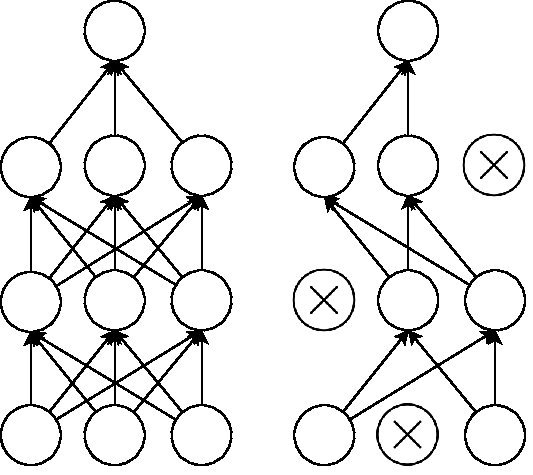
\includegraphics[width=0.5\textwidth]{./pictures/method/dropout}
            \caption{An example of dropout being performed on different layers
                in a network. Some neurons are left out during the forwards and
                backwards pass. To the left the network is shown before dropout
                and to the right after dropout.}
            \label{fig:dropout}
        \end{figure}

        \citet{JMLR:v15:srivastava14a} investigated the use of dropout layers
        in different problem settings. They found that dropout layers reduced
        overfitting in all problems they looked at. In particular interest for
        this thesis, they found that text classification was also improved. The
        main drawback of a dropout layer is that it increase the training time
        of the networks its used on \citep{JMLR:v15:srivastava14a}.

\end{description}


\subsubsection{Training a Network} \label{subsubsec:training_a_network}

A neural network learns by updating the weights in the network. The weights are
updated using \textit{gradient descent} \citep{Bishop}. Gradient descent is
a method that can minimize any differentiable function by taking small steps
towards a local minimum. The function we minimize in a neural network is an
error function. The error function describes a quantity which when minimized
gives the network the best performance possible. Since gradient descent works
for any differentiable function the error function can be any function that is
differentiable. As an example consider the error function,

\begin{align}
    E(W)   &= \sum_{n=1}^{N} E_n(W) \\
    E_n(W) &= \frac{1}{2} \left( \hat{y}_n - y_n \right)^2
\end{align}

where $N$ is the number of training samples, $\hat{y}_n$ is the predicted
results, $y_n$ is the target result, and $W$ is a set of weights. The gradient
is a multi-variable generalization of the derivative of a function. It is a
vector that points in the direction of steepest ascend in value for a function
at a specific point. Gradient descent is based on the observation that a
differentiable function $f$ in point $\mathbf{x}$ decrease fastest in the
direction of the negative gradient of the point $\mathbf{x}$ \citep{Bishop}.
That leads to a simple update rule that can be applied continuously to reach a
local minimum,

\begin{equation}
    \mathbf{x}_{n+1} = \mathbf{x}_n - \eta \Delta f\left(\mathbf{x}_n\right),
\end{equation}

where $\eta$ is a small number that makes sure we do not overstep the local
minimum. An example of the gradient descent process can be seen in Figure
\ref{fig:gradient_descent}. The only parameters we can change in order to
minimize an error function are the weights $\mathbf{w}$. These can be changed by
using the gradient descent update rule,

\begin{figure}
    \centering
    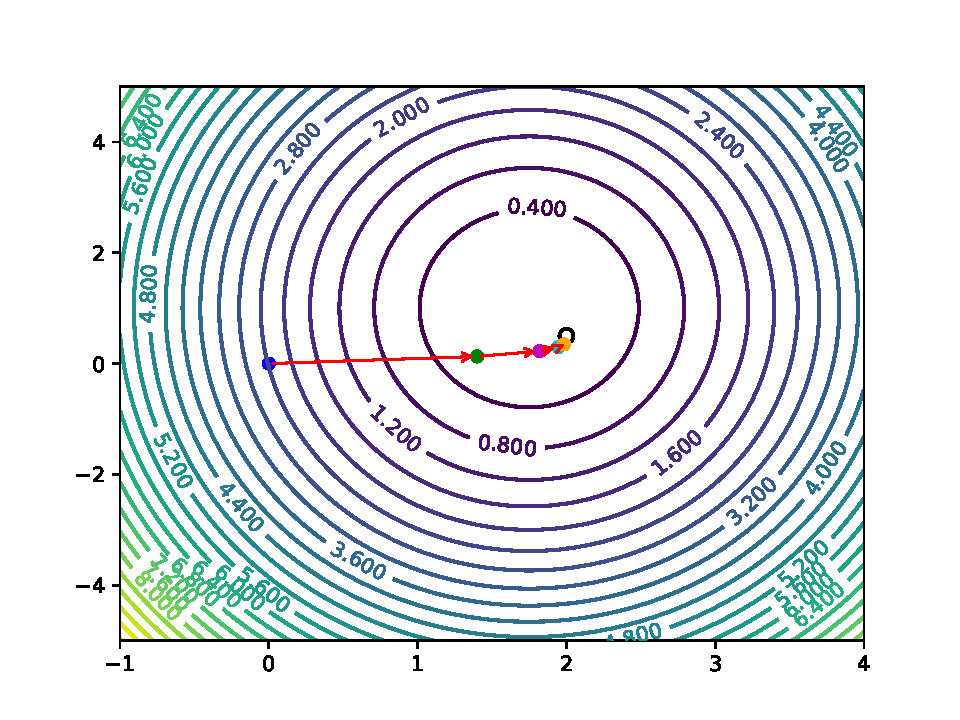
\includegraphics[width=0.8\textwidth]{./pictures/method/gradient_descend}
    \caption{An illustration of how gradient descent works. Each iteration takes
        a step in the direction of the local minimum of the specific function
        used, which in this case is signified by a black ring. The Figure is
        generated using code from
        \url{https://scipython.com/blog/visualizing-the-gradient-descent-method/}.}
    \label{fig:gradient_descent}
\end{figure}

\begin{equation} \label{eq:gradient_descent_network_update}
    \mathbf{w}^{(t+1)} = \mathbf{w}^{(t)} + \eta \Delta \mathbf{w}^{(t)},
\end{equation}

where $t$ is the timestep of the update and,

\begin{equation}
    \Delta \mathbf{w}^{(t)} = -\nabla E|_{\mathbf{w}^{(t)}}.
\end{equation}

$\nabla E|_{\mathbf{w}^{(t)}}$ refers to the gradient of the error function
relative to the specific weight vector $\mathbf{w}^{(t)}$, or rewritten,

\begin{equation}
    \nabla E|_{\mathbf{w}^{(t)}} = \frac{\partial E}{\partial \mathbf{w}^{(t)}}.
\end{equation}

Now we have an update rule for the weights of the network that will minimize an
error function $E$ chosen by us. We can choose $E$ as any function we desire
as long as it is differentiable. The only problem left is how to compute the
gradient of the network. The computation of the gradient can be done via the
backpropagation algorithm \citep{Bishop}. Backpropagation depends on the
activation of all neurons in the network. That gives us a three step algorithm
for updating the weights of the network.

\begin{description}
    \item[Feed Forward] Give input to first layer in network computing the
        activation of all neurons to that specific input.
    \item[Back Propagate] Use the backpropagation algorithm to compute the
        gradient of the network.
    \item[Update Weights] Use gradient descent to update the weights of the
        network.
\end{description}

The computation of the gradient starts at the error function $E$. For
simplicities sake we focus on only a single training sample and fix $E$ as,

\begin{equation}
    E = \frac{1}{2}(\hat{y} - y)^2.
\end{equation}

As mentioned we want to determine the gradient of this with respect to all the
weights in our network $w_{ij} \in W$. In order to do that we need to find
partial derivatives for those same weights and since each specific weight is
tied to a specific neuron we need to differentiate the entire network. But
before doing so, we need to establish the chain rule.

\begin{lemma}[Chain Rule]
\label{lemma:chainrule}

    If functions $f$ and $g$ are both differentiable and $F$ is the composite
    function defined by $F(x) = f(g(x))$, then $F' = f'(g(x)) \cdot g'(x)$,

\end{lemma}

The reason we need of the chain rule is that the loss function is essentially
a chain of function calls that spans the entire network. This fact becomes
apparent when we attempt to evaluate our single sample error function $E$ with
respect to a weight $w_{ij}$. If we keep in mind that the neurons in feed
forward neural networks computes a weighted sum of its inputs as per $a_i$ in
Equation \eqref{eq:neuron}. We know that $E$ only depends on $w_{ij}$ through
the call of $a_i$, and it is for that reason what we can apply the chain rule to
get the following,

\begin{equation}
    \label{eq:bp_start}
    \frac{\partial E}{\partial \mathbf{w}_{ij}} = \frac{\partial E}{\partial a_i}
    \frac{\partial a_i}{\partial \mathbf{w}_{ij}}.
\end{equation}

We can add a little extra notation, which we will use hence forth, for the
sake of easing understanding,

\begin{equation}\label{eq:delta}
    \delta_i = \frac{\partial E}{\partial a_i}.
\end{equation}

$\delta$ is often referred to as the \textit{error} of a specific neuron.
From Equation \eqref{eq:neuron} we get that,

\begin{align}
    \frac{\partial a_i}{\partial \mathbf{w}_{ij}}
        &= \frac{\partial}{\partial \mathbf{w}_{ij}}
            \sum_{m=1}^d \mathbf{w}_{im} x_m + \mathbf{w}_{i0}\\
        &= \frac{\partial}{\partial \mathbf{w}_{ij}} \sum_{m = 0}^d
            \mathbf{w}_{im} x_m\\
        &= x_j.
\end{align}

Notice that we exchanged the $j$ counter in Equation \eqref{eq:neuron} with $m$
since we would otherwise have a name clash. That equation when combined with
Equation \eqref{eq:bp_start} gives us,

\begin{equation} \label{eq:deriv}
    \frac{\partial E}{\partial \mathbf{w}_{ij}} = \delta_i x_j.
\end{equation}

So the derivative of the cost function with respect to the weight
$\mathbf{w}_{ij}$ is simply the value of $\delta$ for a neuron multiplied by
$x$ the input end of the weight for that same neuron. This leaves us with
calculating $\delta_i$ for the hidden units, and the output units of the
network. By differentiating the error function we know that for output units
$\delta$ is computed as,

\begin{equation}
    \label{eq:output}
    \delta_k = \hat{y}_k - y_k,
\end{equation}

where $k$ refers to a specific output neuron. For the hidden units the chain
rule has to be used again,

\begin{equation}
    \label{eq:bp}
    \delta_i = \frac{\partial E}{\partial a_i} =
    \sum_k \frac{\partial E}{\partial a_k} \frac{\partial a_k}{\partial a_i},
\end{equation}

Where the sum runs over all $k$ units $i$ outputs to. The Equation can be
rewritten using the prior established equalities and the chain rule,


\begin{align}
    \sum_k \frac{\partial E}{\partial a_k} \frac{\partial a_k}{\partial a_i}
    &= \sum_k \delta_k \frac{\partial a_k}{\partial a_i}
    & \text{By Equation \eqref{eq:delta}}
    \\
    &= \sum_k \delta_k \frac{\partial a_k}{\partial z_i}
        \frac{\partial z_i}{\partial a_i}
    & \text{By Equation \eqref{eq:neuron} and Lemma \ref{lemma:chainrule}}
    \\
    &= \sum_k \delta_k h'(a_i) \frac{\partial a_k}{\partial z_i}
    \\
    &= \sum_k \delta_k h'(a_i) \left( \frac{\partial}{\partial z_i}
        \sum_{j} \mathbf{w}_{kj} z_j\right)
    \\
    &= \sum_k \delta_k h'(a_i) \mathbf{w}_{ki}
    \\
\end{align}

This highlights that changes in $a_i$ only influences the error-function,
through variations of the variables $a_k$. We can compute the $\delta$ for a
particular hidden unit by backpropagating the $\delta$ value back from higher up
in the network.

As such, we can summarize the weight updating algorithm as,

\begin{enumerate}
    \item

        Provide the network with some input data $\mathbf{x}_n$, and compute the
        activations of each hidden and output neuron using Equation
        \eqref{eq:neuron},

    \item

        Compute $\delta_n$ for each of the output neurons using Equation
        \eqref{eq:output},

    \item

        Back propagate $\delta$s using Equation \eqref{eq:bp} to compute
        $\delta_i$ for each neuron,

    \item

        Use Equation \eqref{eq:deriv} to evaluate the required derivatives, and

    \item

        Update the weight using the computed derivatives
        and the gradient descent update rule from Equation
        \eqref{eq:gradient_descent_network_update}.

\end{enumerate}

These five steps are repeated throughout the training cycle of the neural
networks. Such that the weights are optimized after each full parse over the
training dataset.

The process described above can be computed in linear time ($O(W)$). However,
this is only the case when we are using a singular training sample. The process
has to be repeated for each training sample. The runtime then becomes $O(N\cdot
W)$ where $N$ denotes the total number of training samples. During the normal
training process that is further repeated in a number of epochs $\mathcal{E}$
which in turn further increases the time-complexity to $O(\mathcal{E}\cdot
N\cdot W)$. Even though the runtime is still linear the number of weights might
be huge leading to very long weight update times. Therefore backpropagation and
neural networks might not seem like a viable option \cite{Bishop}.

There is however ways to improve the runtime. Both \textit{stochastic gradient
descent} and its variation \textit{stochastic minibatch gradient descent}
attempt to alleviate this problem by reducing the number of needed epochs
$\mathcal{E}$. A more detailed description can be found in the next Section.
\citet{Bishop} does present other alternatives in his book but none working as
well which is why that is the default approach for neural network frameworks
such as Tensorflow/Keras.


\subsubsection{Optimizers}\label{subsubsec:optimizers}

Traditional gradient descent has been updated with several different algorithms.
These algorithms are called \textit{optimizers}. A good optimizer algorithm
will reach a local minimum faster than traditional gradient descent. The first
optimizer algorithm we will discuss is the \textit{stochastic gradient descent}
algorithm. In the traditional gradient descent we have described a single
weight update require computing the gradient of the error function on each
training sample. Often such a detailed gradient is not needed in practise.
Stochastic gradient descent is an attempt at estimating the gradient of all
datapoints using only a single datapoint. That means that in stochastic gradient
descent weights are updated much more often and is updated on a noisy target
\citep{Bishop}. The advantage of stochastic gradient descent is that convergence
to a local minimum might be much quicker since the algorithm does not have to
go through all training samples for each weight update. The weight updating for
stochastic gradient descent is computed as,

\begin{equation}
    \mathbf{w}^{(t+1)} =
        \mathbf{\mathbf{w}}^{(t)} -
        \eta\Delta E_n|_{\mathbf{w}^{(t)}}.
\end{equation}

In practise each weight update in are computed not based on a single
training sample but on some small number of training samples. That
allows the computation to take advantage of highly optimized matrix
libraries and making each update on a slightly less noisy target
\footnote{\url{http://ufldl.stanford.edu/tutorial/supervised/OptimizationStochas
ticGradientDescent/}}. The version of stochastic gradient descent that use more
than one sample per weight update is known as stochastic minibatch gradient
descend.

To see how stochastic gradient descent might lead to faster convergence consider
a dataset with some number of training samples. To create redundancy in the
dataset we copy all training samples in the dataset to create a new dataset of
twice the size. In classical gradient descent the only effect will be that the
error increases by a magnitude of 2 but will take twice as long to compute.
While stochastic gradient descent will converge at the exact same speed as each
minibatch will still represent an estimate of the true underlying function and
each weight update still takes the same amount of time \citep{Bishop}.

Another advantage of the stochastic method is that the optimizer might escape
from a non optimal local minima and reach a better local minima. To see why that
might happen consider the fact that each minibatch consist of a different subset
of training samples. Even though when computed on all training samples the
gradient points towards the non-optimal local minima the gradient of a single
batch might point towards a better local minima. Therefore the optimizer has the
possibility of following the gradient of single batches that leads to a final
better local minima \citep{Bishop}.

A problem in the stochastic gradient descent algorithm is the need to choose
the learning rate $\eta$. If the learning rate is too high the algorithm
will diverge and if it is to low it will be very slow to converge. Therefore
several extensions to basic stochastic gradient descent has been developed that
automatically tunes the learning rate $\eta$. We will discuss three different
extension \gls{AdaGrad}, \gls{RMSProp} and \gls{Adam}.

In the description of those three algorithms we will slightly abuse vector
notation. Given $\mathbf{a}, \mathbf{b} \in \mathbb{R}^n$ we will keep using
$\mathbf{a} \otimes \mathbf{b}$ to mean an elementwise multiplication but
besides that we use $\frac{\mathbf{a}}{\mathbf{b}}$ to mean an elementwise
division, $\sqrt{\mathbf{a}}$ to mean an elementwise square root and
$\mathbf{a}^n$ to mean an elementwise power.

\begin{description}

    \item[\gls{AdaGrad}:]

        The algorithm was invented by \citet{Duchi:2011:ASM:1953048.2021068}.
        The algorithm attempts to solve the problem of choosing a learning
        rate and the problem of how to handle parameters that are infrequently
        activated. When a parameter is only infrequently activated the gradient
        on that parameter will often be close to 0. Infrequently used parameters
        are often the most important parameters for a classification task but
        since they are infrequent they are hard to learn on. \gls{AdaGrad}
        assigns a separate learning rate to each separate parameter. The
        algorithm gives infrequently observed parameters a very high learning
        rate and frequently observed parameters a very low learning rate. The
        method incorporates knowledge of the data from previous iterations to
        make choices in the current iteration. In \gls{AdaGrad} the weight
        update function is,

        \begin{equation}
            \mathbf{w}^{(t+1)} =
                \mathbf{w}^{(t)} -
                \eta \text{diag}\left(G^{(t)}\right)^{-\frac{1}{2}} \otimes
                \Delta E|_{\mathbf{w}^{(t)}},
        \end{equation}

        where $G^{(t)}$ is a matrix containing the sum of the outer product
        of the gradient in all previous timesteps $1, \dots, t$ and
        $\text{diag}(X)$ is the diagonal vector of the matrix $X$. $G^{(t)}$ is
        defined as,

        \begin{equation}
            G^{(t)} = \sum_{t'=1}^t \Delta E|_{\mathbf{w}^{(t')}}
                \left(
                    \Delta E|_{\mathbf{w}^{(t')}}
                \right)^T.
        \end{equation}

        For the updating of a single weight $w_i$ the above becomes
        \citep{Duchi:2011:ASM:1953048.2021068},

        \begin{equation}
            \label{eq:individual_adagrad}
            \mathbf{w}_i^{(t+1)} =
                \mathbf{w}_i^{(t)} - \frac{\eta}{\sqrt{G^{(t)}_{ii}}}
                \Delta E|_{\mathbf{w}_i^{(t)}}.
        \end{equation}

        $G_{ii}$ works as a scaling factor for weight $\mathbf{w}_i$.
        Since $\sqrt{G_{ii}} = \sqrt{\sum_{t'=1}^t \left(\Delta
        E|_{\mathbf{w}^{(t')}_i}\right)^2}$, $G_{ii}$ is the L2 norm of the
        gradient in the previous timesteps. That means that if the gradient
        has generally been large for a particular weight the norm will be
        large and the updating of the weight will be scaled down (slower)
        which can be seen in Equation \eqref{eq:individual_adagrad}. Similarly
        when the gradients of a weight has been small or 0 the weight is
        scaled less down and the upgrade will be larger. That has the effect
        of having infrequently activated parameters of the model train faster
        \citep{Duchi:2011:ASM:1953048.2021068}.

    \item[\gls{RMSProp}:]

        \gls{RMSProp} was introduced by Geoff Hinton in lecture 6e of his
        Coursera Class \citep{DBLP:journals/corr/Ruder16}. This section is based
        primarily on his slides \citep{HintonSrivastavaSwersky2014}. The idea
        behind \gls{RMSProp} is similar to \gls{AdaGrad} each weight is updated
        at an independent rate. Unlike \gls{AdaGrad} the rate is chosen by a
        moving average instead of the L2 norm of all previous steps. That allows
        the algorithm to adapt quickly to changes in the gradient. When the
        gradient of a weight is large the algorithm decreases the learning rate
        and when the gradient is consistently small it tunes up the learning
        rate. That functions well since a large gradient is found in a steep
        volatile area while a consistently small gradient is found in a flat non
        volatile area. In the steep areas we are likely to overshoot the target
        if the learning rate is to high while in flat areas we do not have that
        problem. The internal state of the algorithm is a vector $\mathbf{v}$
        containing the running average of gradient magnitudes. It is updated
        with the equation,

        \begin{equation}
            \label{eq:rms_prop_state}
            \mathbf{v}^{(t+1)} =
                \gamma\mathbf{v}^{(t)} +
                (1 - \gamma)\left(
                    \Delta E|_{\mathbf{w}^{(t + 1)}} \otimes
                    \Delta E|_{\mathbf{w}^{(t + 1)}}
                \right).
        \end{equation}

        The parameter $\gamma$ can be seen as a remembering rate. If $\gamma$
        is high we keep much of the previous running average and if $\gamma$
        is low we update the average much quicker. The actual weight update is
        performed by using the internal state $\mathbf{v}$ to scale the learning
        rate $\eta$,

        \begin{equation}
            \mathbf{w}^{(t+1)} =
                \mathbf{w}^{(t)} -
                \frac{\eta}{\sqrt{\mathbf{v}^{(t)}}} \otimes
                \Delta E|_{\mathbf{w}^{(t)}}.
        \end{equation}

    \item[\gls{Adam}:]

        \gls{Adam} is an upgrade of the \gls{RMSProp} algorithm invented by
        \citet{DBLP:journals/corr/KingmaB14}. The difference from \gls{RMSProp}
        is that \gls{Adam} use both the gradient and the squared gradient while
        \gls{RMSProp} use only the squared gradient. Consequently \gls{Adam} has
        two remembering factors instead of the single one for \gls{RMSProp}. The
        internal state of \gls{Adam} is updated via,

        \begin{align}
            \mathbf{m}^{(t+1)} &=
                \gamma_1\mathbf{m}^{(t)} +
                (1 - \gamma_1) \Delta E|_{\mathbf{w}^{(t)}}, \\
            \mathbf{v}^{(t+1)} &=
                \gamma_2\mathbf{v}^{(t)} +
                (1 - \gamma_2) \left(
                    \Delta E|_{\mathbf{w}^{(t)}} \otimes \Delta E|_{\mathbf{w}^{(t)}}
                \right), \\
            \mathbf{\hat{m}}^{(t+1)} &=
                \frac{\mathbf{m}^{(t+1)}}{1 - \gamma_1^{t + 1}}, \\
            \mathbf{\hat{v}}^{(t+1)} &=
                \frac{\mathbf{v}^{(t+1)}}{1 - \gamma_2^{t + 1}}.
        \end{align}

        The first two equations are very similar to Equation
        \eqref{eq:rms_prop_state} for \gls{RMSProp}. In those equations
        $\gamma_1$ and $\gamma_2$ are the remembering rates of the gradient
        and the squared gradient. They keep a running average of the gradient
        and the magnitude of the gradient. By using the running average of
        the gradient \gls{Adam} is able to move more smoothly in a direction
        since the direction chosen is no longer based on just the current
        gradient but on previous gradients as well. That means that a single
        weird gradient will not drastically change the direction \gls{Adam}
        moves \citep{DBLP:journals/corr/KingmaB14}. Similar to \gls{RMSProp},
        \gls{Adam} use the running average of the squared gradient to scale how
        large steps are taken. The two bottom equations are scaling the internal
        state based on the time step $t$. As $t$ increases the denominators
        increase meaning that the value of the whole fraction decreases. That
        means that in the beginning the step size is adjusted upwards and as
        $t$ increases, smaller and smaller steps are taken. The actual weight
        updates in the \gls{Adam} algorithm are then given by,

        \begin{equation}
            \mathbf{w}^{(t + 1)} = \mathbf{w}^{(t)} -
                \eta\frac
                    {\mathbf{\hat{m}}^{(t+1)}}
                    {\sqrt{\mathbf{\hat{v}}^{(t+1)}} + \epsilon}.
        \end{equation}

        \gls{Adam} prevents division by 0 via the $\epsilon$ parameter which is
        just some small number. It can be seen in the above equation that the
        direction of change is chosen by $\mathbf{\hat{m}}^{(t)}$ while the size
        of the step taken is chosen by a combination of the learning rate $\eta$
        and $\mathbf{\hat{v}}^{(t)}$.

        \gls{Adam} has been found to work great for \gls{NLP} tasks
        \cite{Pompey2016TheAO}. The main advantage \gls{Adam} has with regard
        to \gls{NLP} would be the properties it inherits from \gls{AdaGrad}.
        This allows for more focus to be placed upon the less activated
        parameters. Text data generally have many features that are rarely seen
        but when they are they are great indicators of authorship. Therefore
        separate learning rates are important. The running average scaling that
        \gls{RMSProp} introduces makes sure that \gls{Adam} can quickly adopt to
        new situations.

\end{description}


\subsubsection{Siamese Networks}\label{subsubsec:siamese_networks}

Classical machine learning approaches for text analysis and all our
baseline methods are based on handcrafted feature sets. Deep learning
has shown promising results in extracting features from raw images and
raw text \citep{hongxiaosunyuan}. We wanted to use deep learning to
automatically learn features from a large amount of raw data. At the
same time we wanted to solve the MaCom authorship verification problem.
Siamese neural networks are as described earlier networks that compares
two inputs. They have been used for comparing texts, images and signatures
\citep{Koch2015SiameseNN,NIPS1993_769,qian:2018}. \citet{qian:2018} use a
Siamese network but with no convolutions and a distance function on top for
text analysis while \citet{Koch2015SiameseNN} used a siamese network with
convolutions and fully connected network on top for image analysis. Our approach
is to use convolutions or \gls{RNN}s in the siamese network to learn important
features from the texts. We also use a fully connected network on top of the
feature extraction layers to learn from the features the extracted. An example
of this architecture can be seen in Figure \ref{fig:siamese_example}.

\begin{figure}
    \centering
    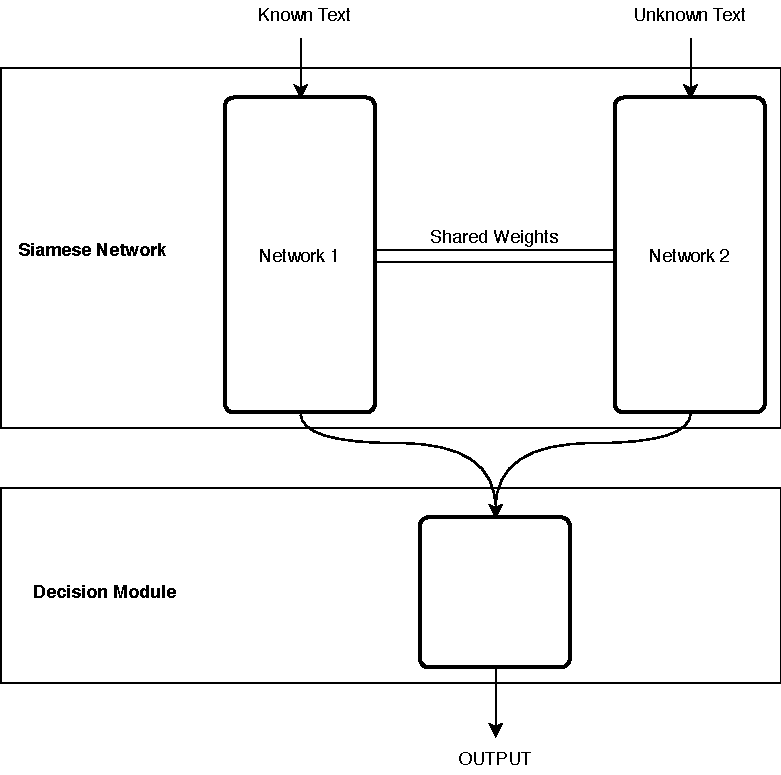
\includegraphics[scale=0.5]{./pictures/method/siamese}
    \caption{The basic architecture of a siamese neural network. The network
        takes two sources of data and runs it through two parallel weight
        sharing networks. The two parallel networks extracts features from the
        raw data. Those features are given to a prediction module that compares
        the feature sets extracted. The decision module can be anything that
        compares two vectors such as a distance function or a dense neural
        network.}
    \label{fig:siamese_example}
\end{figure}

The network will take two inputs, a text $t \in T_\alpha$ and a text $t' \in
T_{\alpha'}$. The network will then try to determine whether $\alpha = \alpha'$
by comparing $t$ and $t'$. The siamese part of the network will extract features
from the texts using convolutions or \gls{RNN} layers. These features will serve
as a \textit{representation} of the texts $t$ and $t'$. This representation will
be given to a dense network which will learn how to compare the feature sets
extracted.

\citet{DBLP:journals/corr/0001KYS17} presented a comparative study of
\glspl{CNN} and \glspl{RNN} in common \gls{NLP} tasks. They found that
\glspl{RNN} generally performed better in tasks where understanding the whole
text was important while \glspl{CNN} performed better when understanding was
secondary and the goal was mainly about finding key phrases or statistical
information from a text. In authorship verification the understanding of the
text is generally irrelevant since we do not have to say anything about what a
text is about but only whether or not it is written by the same author as some
other text. Furthermore classical authorship verification methods have relied on
statistical information from the texts and not on an actual understanding of the
texts. Therefore we started experiments by using \glspl{CNN}.

The final output of the networks we train will be the probability that $\alpha =
\alpha'$. Since the MaCom dataset consist of multiple texts per author and this
network architecture only compares two texts we define a separate system for
making the final prediction based on all $t \in T_\alpha$.


\subsection{Combining Neural Network Output}
\label{subsec:combining_neural_network_output}

In the generic Siamese neural network presented in Section
\ref{subsubsec:siamese_networks} the output of the network is a probability
that two texts are written by the same author. However in the problem we are
trying solve defined in Definition \ref{def:authorship_verification} we take
several texts as input. We therefore need a method of combining the predictions
on multiple texts to a single prediction on a particular problem instance. We
do that using a \textit{prediction system}. We let the generic siamese neural
network described above be known as a \textit{text comparison function} $f \in
\mathcal{F}$.

\begin{definition}[Text Comparison Function]
    \label{def:text_comparison_function}

    Let $\mathcal{F} \colon \mathcal{T} \times \mathcal{T} \rightarrow [0, 1]$
    be any function that compares two texts and outputs the probability that the
    the texts are written by the same author.

\end{definition}

For fixed text comparison function $f$, we now define the \textit{weighted
average based prediction system} $P_w$.

\begin{definition}[Weighted Average Prediction System]
    \label{def:weighted_average_prediction_system}

    Let $w: \mathcal{T} \rightarrow [0, 1]$ be a weight function, such that
    $\forall \alpha \in \mathcal{A}: \sum_{t \in T_\alpha} w(t) = 1$. Then the
    weighted average prediction system is given by,

    \begin{align}
        &P_w \colon \mathcal{A} \times \mathcal{T} \times [0, 1] \rightarrow
            \{0, 1\} \\
        &P_w(\alpha, t, \theta) \mapsto \mathbbm{1}\left[
                \sum_{t' \in T_\alpha} w(t') f(t, t') > \theta
            \right],
    \end{align}

    where $\mathbbm{1}\left[\cdot\right]$ is the indicator function.

\end{definition}

That is, the weighted average prediction system $P_w$ returns 1 if the weighted
average of the probability that $t$ is written by the same author as $t'$ for
each $t' \in T_\alpha$ is greater than the threshold $\theta$ and 0 otherwise.

The $\theta$ parameter in $P_w$ determines when we consider an unknown text
to be written by an author. The $\theta$ parameter can be used to enforce how
sure we have to be of a decision to accuse an author of not having written
an assignment. As described earlier MaCom does not want to accuse innocent
students of cheating. That means that it is very important to minimize the
accusation error. We can use the $\theta$ parameter to control that error.

The $w$ parameter in the prediction system can be used to weigh the texts
a claimed author has written. We are going to try several different weight
functions that weigh texts based on metadata such as the time they were written
and the length of the texts. In the following definition of different weight
functions we will ignore the constraint that the weight functions has to sum to
1 for each author. We ignore that constraint since for any weight function $w
\colon \mathcal{T} \rightarrow \mathbb{R}$ we can define a new weight function
$w^* \colon \mathcal{T} \rightarrow [0, 1]$ as,

\begin{equation}\label{eq:normalize}
    w^*(t) = \frac{w(t)}{\sum_{t' \in T_\alpha} w(t')}.
\end{equation}

We can therefore define the weight functions $w$ while ignoring the constraint
but use $w^*$ as the actual weight function in the weighted prediction system.

The most obvious weighing scheme is to just use a uniform weighting. That way
we simply take an average of the predictions of our networks over the different
texts an author has written.

\begin{definition}[Uniform Weight]
    \label{def:uniform_weight}

    The uniform weight function is given by,

    \begin{align}
        &u \colon \mathcal{T} \rightarrow \{ 1 \} \\
        &u(t) \mapsto 1.
    \end{align}

\end{definition}

The \textit{uniform weight} function does not use any information we know about
the texts. We define it as a baseline to make sure we do not make any weight
functions that are worse than a simple uniform weighing. Our other weight
functions use metadata we know about the texts. We start by defining a weight
function \textit{exponential dropoff weight} that use the time a text was turned
in to MaCom's servers to weight the texts. We assume that newer texts will
better reflect the current writing style of a student than older texts. Recall
that $\tau$ denotes the function that returns the relative time of a text as
described in Section \ref{subsec:notation}.

\begin{definition}[Exponential Dropoff Weight]
    \label{def:exponential_dropoff_weight}

    Given $\lambda \in \mathbb{R}^+$ the time based exponential dropoff weight
    function is given by,

    \begin{align}
        &exp_\lambda \colon \mathcal{T} \rightarrow \mathbb{R}^+ \\
        &exp_\lambda(t) \mapsto e^{-\lambda \tau(t)}.
    \end{align}

\end{definition}

The $\lambda$ parameter can be used to control how important newer texts are.
When $\lambda = 0$ the exponential dropoff weight is equivalent to the Uniform
Weight function and as $\lambda \rightarrow \infty$ more weight is given to
the most recent texts. We have shown the weights given to different texts for
different $\lambda$ values in Figure \ref{fig:weights}.

\begin{figure}
    \centering
    \textbf{Exponential Dropoff Weights}\par\medskip
    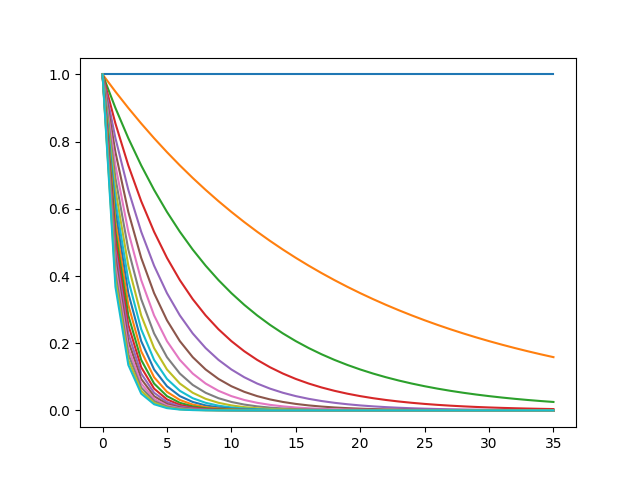
\includegraphics[width=0.49\textwidth]{./pictures/method/weights.png}
    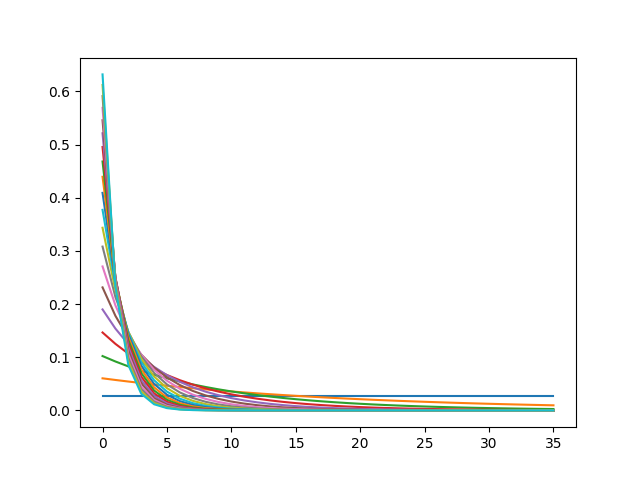
\includegraphics[width=0.49\textwidth]{./pictures/method/weights_normalized.png}
    \caption{Illustrate the exponential dropoff weight function for different
    values of $\lambda$. We apply the weight function to the numbers $0, 1,
    \dots, 35$ since a typical student will attend secondary school for 3 years
    (36 months). On the left the pure output of the weight function $w_e$ is
    shown and on the right the normalized weights $w_e^*$. The value of
    $\lambda$ varies from 0 to 1 with step size 0.05.}
    \label{fig:weights}
\end{figure}

We have also defined weight functions that use other metadata besides the time
of writing. Specifically we have used the length of texts. The idea is that
longer texts provide better insight into an authors writing style than shorter
texts. So we wanted to see if we could obtain better results if we considered
text length.

\begin{definition}[Length Weight]

    The text length based weight function is given by,

    \begin{align}
        &l \colon \mathcal{T} \rightarrow \mathbb{N}^+ \\
        &l(t) \mapsto \left\lfloor \frac{|t|}{1000} \right\rceil + 1,
    \end{align}

    where $\lfloor x \rceil$ is $x$ rounded to nearest whole number.

\end{definition}

Thus this weight function gives more weight the longer a text is but where only
differences on the order of thousands of characters are considered significant.
We used the exponential dropoff weight and length weight functions to implement
another weight function that use both text length and time to give weights to
texts.

\begin{definition}[Exponential Dropoff and Length Weight]

    Given $\lambda \in \mathbb{R}^+$ the combined time and length weight
    function is given by,

    \begin{align}
        &lexp_\lambda \colon \mathcal{T} \rightarrow [0, 2] \\
        &lexp_\lambda(t) \mapsto exp^*_\lambda(t) + l^*(t).
    \end{align}

\end{definition}

Which is simply the addition of the exponential dropoff weight and the length
weight, after they are both individually applied to the text.

We have also defined some different prediction systems that are not based on
weighted averages. The first such system is the $P_{max}$ prediction system.
The thought behind the system is that we wanted to minimize the accusation
error. The prediction system takes the text $t' \in T_\alpha$ that looks the
most like $t$. That way if just a single assignment from a candidate author
looks sufficiently like the text we are comparing with we report that the author
matches. That should hopefully result in less people being accused of ghost
writing.

\begin{definition}[Maximum Prediction System]
    \label{def:maximum_prediction_system}

    The maximum prediction system $P_{max}$ based only on most similar text is
    given by,

    \begin{align}
        &P_{max} \colon \mathcal{A} \times \mathcal{T} \times [0, 1] \rightarrow
            \{0, 1\} \\
        &P_{max}(\alpha, t, \theta) \mapsto \mathbbm{1}\left[
                \underset{t' \in T_\alpha}{\text{maximize}} f(t, t') > \theta
            \right].
    \end{align}

\end{definition}

For completeness we also defined a $P_{min}$ prediction system that use only the
least similar text for the prediction. We expect that such a function will be
quick to accuse authors of ghostwriting since it only looks at the one text that
seem to indicate ghostwriting.

\begin{definition}[Minimum Prediction System]
    \label{def:minimum_prediction_system}

    The minimum prediction system $P_{min}$ based only on least similar text is
    given by,

    \begin{align}
        &P_{min} \colon \mathcal{A} \times \mathcal{T} \times [0, 1] \rightarrow
            \{0, 1\} \\
        &P_{min}(\alpha, t, \theta) \mapsto \mathbbm{1}\left[
                \underset{t' \in T_\alpha}{\text{minimize}} f(t, t') > \theta
            \right].
    \end{align}

\end{definition}

Finally we also defined a prediction system that takes a majority vote. The
majority vote is similar to a uniform weight function. The difference is that
the majority vote does not use the actual value of a prediction but only how
many are on each side of a threshold. As an example assume that an author
$\alpha$ has written three texts $\{t_1, t_2, t_3\} = T_\alpha$ and we are
comparing to text $t$ with $\theta = 0.5$. Let us then assume that $f(t, t_1)
= 0.0$, $f(t, t_2) = 0.51$ and $f(t, t_3) = 0.51$. Then the uniform weight
function would compute $\mathbbm{1} \left[ \frac{1}{3} 0.0 + \frac{1}{3} 0.51 +
\frac{1}{3} 0.51 > 0.5 \right] = 0$. Meaning that the author would be accused
of using a ghostwriter even though two of his assignments are more similar than
dissimilar. Contrary to that a majority vote would report 1 since more texts are
greater than $\theta$ than lower.

\begin{definition}[Majority Vote Prediction System]
    \label{def:majority_vote_prediction_system}

    The majority vote prediction system $P_{MV}$ is given by,

    \begin{align}
        &P_{MV} \colon \mathcal{A} \times \mathcal{T} \times [0, 1] \rightarrow
            \{0, 1\} \\
        &P_{MV}(\alpha, t, \theta) \mapsto \mathbbm{1}\left[
                \frac{1}{|T_\alpha|} \sum_{t' \in T_\alpha} \mathbbm{1}\left[
                    f(t, t') > \theta
                \right] > \frac{1}{2}
            \right].
    \end{align}

\end{definition}


\subsubsection{Tuning Parameters}
\label{subsubsec:tuning_parameters}

The prediction systems defined above has several hyperparameters we have to
choose to get the best results. We recall that MaCom wanted a system that
had an accusation error of less than 10\%. We can use the shared threshold
parameter $\theta$ in the prediction systems to control how many people we
accuse. The best parameters for the prediction systems is those parameters that
gives the highest accuracy subject to the 10\% accusation error constraint. To
tune the parameters we use a validation dataset not seen during training. From
that dataset we construct a set of tuples $(\alpha, t_u)$ where $\alpha$ is a
candidate author and $t_u$ is a text of unknown authorship. We let the set of
tuples be known as $V$. The parameters that maximize the accuracy subject to the
bounded accusation error is the same as the parameters that minimize the error
rate subject to the bounded accusation error. That optimization problem is,

\begin{equation}
    \label{eq:prediction_system_minimization}
    \begin{aligned}
        & \underset{\theta, x}{\text{minimize}}
        & & \sum_{(\alpha, t_u) \in V} \left|
            P_x(T_\alpha \setminus \{t_u\}, t_u, \theta) -
            \mathbbm{1}\left[t_u \in T_\alpha\right]
        \right| \\
        & \text{subject to}
        & & \frac{\sum_{(\alpha, t_u) \in V} \mathbbm{1}\left[t_u \in T_\alpha\right] \cdot
            \left(1 - P_x(T_\alpha \setminus \{t_u\}, t_u, \theta)\right)}
{\sum_{(\alpha, t_u) \in V} (1 - P_x(T_\alpha \setminus \{t_u\}, t_u, \theta)} <
            \frac{1}{10}
    \end{aligned}
\end{equation}

In the optimization problem we fix the network $f$ like we did when defining
the prediction systems. The expression we minimize is the number of errors made
in prediction over the validation set $V$. Consider a problem $(\alpha, t_u)
\in V$ where $t_u \in T_\alpha$. Then we know that $\mathbbm{1}\left[t_u \in
T_\alpha\right] = 1$ from the definition of the indicator function then if the
prediction system returns the correct result 1 we have,

\begin{equation}
    e = \left|
        P_x(T_\alpha \setminus \{t_u\}, t_u, \theta) -
        \mathbbm{1}\left[t_u \in T_\alpha\right]
    \right| = |1 - 1| = 0,
\end{equation}

and if the prediction system returns the incorrect result 0 we have,

\begin{equation}
    e = \left|
        P_x(T_\alpha \setminus \{t_u\}, t_u, \theta) -
        \mathbbm{1}\left[t_u \in T_\alpha\right]
    \right| = |0 - 1| = 1.
\end{equation}

Similarly for a problem $(\alpha, t_u) \in V$ where $t_u \notin T_\alpha$ we
know that $\mathbbm{1}\left[t_u \in T_\alpha\right] = 0$ from the definition of
the indicator function. Then if the prediction system returns the correct result
0 we have,

\begin{equation}
    e = \left|
        P_x(T_\alpha \setminus \{t_u\}, t_u, \theta) -
        \mathbbm{1}\left[t_u \in T_\alpha\right]
    \right| = |0 - 0| = 0, \end{equation}

and if the prediction system returns the incorrect result 1 we have,

\begin{equation}
    e = \left|
        P_x(T_\alpha \setminus \{t_u\}, t_u, \theta) -
        \mathbbm{1}\left[t_u \in T_\alpha\right]
    \right| = |1 - 0| = 1.
\end{equation}

That is the expression we minimize is 0 whenever there is no error and 1
whenever there is an error. So we minimize the number of errors we make. The
subject to expression makes sure that the fraction of false accusations we make
is less than $10\%$ of the accusations we make. The expression should be read
as,

\begin{equation}
    \frac{\textit{false accusations}}{\textit{total accusations}} < \frac{1}{10}
\end{equation}

Consider the numerator of the fraction on the left hand side,

\begin{equation}
    \textit{false accusations} = \sum_{(\alpha, t_u) \in V}
    \mathbbm{1}\left[t_u \in T_\alpha\right] \cdot
    \left(1 - P_x(T_\alpha \setminus \{t_u\}, t_u, \theta)\right).
\end{equation}

For a $(\alpha, t_u) \in V$ where $t_u \in T_\alpha$ we have that
$\mathbbm{1}\left[t_u \in T_\alpha\right] = 1$ then if $P$ is correct it returns 1 and we
get,

\begin{equation}
    \mathbbm{1}\left[t_u \in T_\alpha\right] \cdot
    \left(1 - P_x(T_\alpha \setminus \{t_u\}, t_u, \theta)\right) =
    1 \cdot (1 - 1) = 0,
\end{equation}

and if $P$ is incorrect and returns 0 we have,

\begin{equation}
    \mathbbm{1}\left[t_u \in T_\alpha\right] \cdot
    \left(1 - P_x(T_\alpha \setminus \{t_u\}, t_u, \theta)\right) =
    1 \cdot (1 - 0) = 1.
\end{equation}

Similarly for a $(\alpha, t_u) \in V$ where $t_u \in T_\alpha$ we have that
$\mathbbm{1}\left[t_u \in T_\alpha\right] = 0$ and therefore the expression is
always 0. Therefore the expression is 1 whenever we have a false accusation
and 0 otherwise. The denominator of the fraction simply counts the number of
accusations by inverting the output of $P_x$. Since that fraction has to be
below $\frac{1}{10}$ we make sure that only 10\% of the accusations we make are
false accusations.

In the real world it has been estimated that 4\% of turn
ins for the \gls{SRP} are written by "ghostwriters"
\footnote{https://politiken.dk/indland/uddannelse/art5603163/Gymnasieelever-\%C2
\% BBSnyderi-beviser-hvor-vanvittig-betydningsfuld-SRP-er-blevet\%C2\%AB}.
We therefore want to find the best prediction system and threshold $\theta$
on a dataset with 4\% negatives. We also find the best prediction system and
threshold for a dataset with 50\% negatives as that is easier to compare with
other methods.


\subsection{Summary}

To summarize we will implement 2 baseline methods and an indeterminate number of
neural network based methods. The baseline methods will be the extended delta
method and an author specific \gls{SVM} method. The baselines will both need
manually extracted feature sets and feature tuning. The networks will be siamese
neural networks. They work by using either convolutional or recurrent networks
to extract features from raw text data. The features are compared using a dense
network. Each of our neural networks will only compare two texts at a time.
Since an author has multiple texts we will combine the predictions on each of
an author's texts using a prediction system. We will find the best prediction
system and parameters using a validation set.
